\documentclass{sig-alternate-05-2015}
\usepackage{tabularx,colortbl}
\usepackage[dvipsnames]{xcolor}
\usepackage{flushend}
\usepackage{cite}
\usepackage{amsmath}
%\usepackage{amsthm}
\usepackage{amssymb}
\usepackage{epsfig}
\usepackage{stmaryrd}
\usepackage{url}
\usepackage{multirow}
\usepackage{latexsym}
\usepackage{graphics}
\usepackage{graphicx}
\usepackage{enumitem}
\usepackage{comment}
\usepackage{longtable}
\usepackage{supertabular}
\usepackage{times}
\usepackage{listings}
\usepackage{subfigure}
\usepackage{color}
\usepackage{balance}
\usepackage[ruled, vlined, linesnumbered]{algorithm2e}



%\theoremstyle{Definition}
%\newtheorem{definition}{Definition}
%%
%\theoremstyle{Theorem}
%\newtheorem{theorem}{Theorem}


%\newcommand{\definition}{\noindent \textbf{Definition} \citation{}}
%\newcommand{\theorem}{\noindent \textbf{Theorem} \citation{}}
%\newcommand{\lemma}{\noindent \textbf{Lemma} \citation{}}

\newcommand{\mkeyword}[1]{\mbox{\texttt{#1}}}
\DeclareMathOperator{\kuop}{uop}
\DeclareMathOperator{\kbop}{bop}
\DeclareMathOperator{\kite}{ite}
\DeclareMathOperator{\kpre}{pre}
\DeclareMathOperator{\dom}{dom}
\DeclareMathOperator{\ktrue}{true}
\DeclareMathOperator{\kfalse}{false}
\DeclareMathOperator{\kselect}{select}
\DeclareMathOperator{\ran}{range}
\newcommand{\lbb}{[\![}
\newcommand{\rbb}{]\!]}
\newcommand{\expr}{\phi}
\newcommand{\exprS}{\Phi}
% this toggles between a tech-report version of the paper and the MEMOCODE version
%\newcommand{\TECHREPORT}{}
%\tolerance=1
%\emergencystretch=\maxdimen
%\hyphenpenalty=10000
%\hbadness=10000
\sloppypar



\begin{document}
\CopyrightYear{2016}
\setcopyright{acmcopyright}
\conferenceinfo{FSE'16,}{November 13-19, 2016, Seattle, WA, USA}
\isbn{978-1-4503-4218-6/16/11}\acmPrice{\$15.00}
\doi{http://dx.doi.org/10.1145/2950290.2950346}
 % Add this to every tex file, so that you can comment with a diff color%
\definecolor{gold}{rgb}{0.90,.66,0}
\definecolor{dgreen}{rgb}{0,0.6,0}
\newcommand{\mike}[1]{\textcolor{red}{#1}}
\newcommand{\fixed}[1]{\textcolor{purple}{#1}}
\newcommand{\andrew}[1]{\textcolor{green}{#1}}
\newcommand{\ela}[1]{\textcolor{blue}{#1}}
\newcommand{\stateequiv}{\equiv_{s}}
\newcommand{\traceequiv}{\equiv_{\sigma}}
\newcommand{\ta}{\text{TA}}
\newcommand{\cta}{\text{TA$_{C}$}}
\newcommand{\tta}{\text{TA$_{T}$}}

\newdef{lemma}{Lemma}
\newdef{definition}{Definition}
\newdef{theorem}{Theorem}
\newdef{note}{Note}
%\newcommand{\TECHREPORT}{}

\title{Efficient Generation of All Inductive Validity Cores (IVCs)}

\numberofauthors{3}

\author{
\alignauthor
Elaheh Ghassabani\\
       \affaddr{Department of Computer Science and Engineering}\\
       \affaddr{University of Minnesota}\\
       \affaddr{\small{200 Union Street\\Minneapolis, MN, 55455, USA}}\\
       \email{\texttt{\small{ghass013@umn.edu}}}
\alignauthor
Andrew Gacek\\
       \affaddr{Rockwell Collins\\ Advanced Technology Center}\\
       \affaddr{\small{400 Collins Rd. NE\\Cedar Rapids, IA, 52498, USA}}\\
       \email{\texttt{\small{andrew.gacek@rockwellcollins.com}}}
\alignauthor
Michael W. Whalen\\
       \affaddr{Department of Computer Science and Engineering}\\
       \affaddr{University of Minnesota}\\
       \affaddr{\small{200 Union Street\\Minneapolis, MN, 55455, USA}}\\
       \email{\texttt{\small{whalen@cs.umn.edu}}}
}

\maketitle

\begin{abstract}
All IVCs method is awesome!!!! :-)
\end{abstract}

%\begin{CCSXML}
%<ccs2012>
%<concept>
%<concept_id>10003752.10003790.10003794</concept_id>
%<concept_desc>Theory of computation~Automated reasoning</concept_desc>
%<concept_significance>500</concept_significance>
%</concept>
%<concept>
%<concept_id>10003752.10003790.10011192</concept_id>
%<concept_desc>Theory of computation~Verification by model checking</concept_desc>
%<concept_significance>500</concept_significance>
%</concept>
%<concept>
%<concept_id>10011007.10011074.10011075.10011076</concept_id>
%<concept_desc>Software and its engineering~Requirements analysis</concept_desc>
%<concept_significance>500</concept_significance>
%</concept>
%<concept>
%<concept_id>10011007.10011074.10011099.10011692</concept_id>
%<concept_desc>Software and its engineering~Formal software verification</concept_desc>
%<concept_significance>500</concept_significance>
%</concept>
%</ccs2012>
%\end{CCSXML}
%
%\ccsdesc[500]{Theory of computation~Verification by model checking}
%\ccsdesc[500]{Theory of computation~Automated reasoning}
%\ccsdesc[500]{Software and its engineering~Requirements analysis}
%\ccsdesc[500]{Software and its engineering~Formal software verification}
%\printccsdesc
\keywords{Inductive validity cores, UNSAT-core generation, SMT-based model checking, Inductive proofs}

\section{Introduction}
\label{sec:intro}

In order to build software, one usually starts with {\em requirements}, a set of statements about what the software is intended to do, which is refined either prior to, or in tandem with, the software being developed.  Requirements are necessary to software both for shaping the development of the software and for determining its adequacy when performing verification activities.  Therefore, determining the {\em adequacy} of requirements is of substantial importance to the eventual quality of the software.

Zowghi and Gervasi~\cite{} define adequacy of requirements in terms of the ``three Cs'': Consistency, Completeness, and Correctness.  \mike{[MOST OF THE REST OF THIS PARAGRAPH IS BLATANTLY STOLEN FROM GERVASI - REWRITE]} Davis states that completeness is the most difficult of the specification attributes to
define and incompleteness of specification is the most difficult violation to detect~\cite{}.
According to Boehm~\cite{}, to be considered complete, the requirements document must exhibit three fundamental characteristics: (1) No information is left unstated or ``to be determined'', (2) The information does not contain any undefined objects or entities, (3) No information is missing from this document. The first two properties imply a closure of the existing information and are typically referred to as internal completeness.  The third property, however, concerns the external completeness of the document
\cite{}. External completeness ensures that all of the information required for problem definition is found within the specification.  However, {\em assessing} external completeness in a precise and formal way is difficult, if not impossible, because there is rarely an external reference that can be used to determine whether all relevant requirements have been defined.

What tends to happen instead is that we measure the {\em relative completeness} of requirements with respect to some other artifact.  Usually, the other artifact is some form of implementation of the requirements (it could an abstract ``model'' of the implementation, source code, or object code).  This idea underlies certification standards such as DO178B/C~\cite{}, which require that requirements-based tests are sufficient to achieve structural coverage of the code to a certain level of rigor.  More recent work by Zeller~\cite{} and Murugesan~\cite{} have attempted to adapt these measure towards automated test generation by examining coverage of {\em assertions} in the code.  

A drawback of the approach is that an implementation must exist prior to performing this analysis; if the implementation is only available late in the development process, then incompleteness in requirements is not exposed until very late in the development cycle, potentially leading to substantial rework.  Next, the approach usually requires thousands to hundreds of thousands of tests, which are expensive to construct and can be expensive to modify in the face of changing or incomplete requirements.  Finally, the test metrics that are used for measurement tend to substantially overapproximate which portions of a program are necessary to fulfill a requirement~\cite{} \mike{cite MCDC and OMCDC work here}.

In addition, what happens if we want to use formal methods to prove system requirements?  Arguably, proofs should lead to higher assurance than tests, leading to more confidence in system performance.  However, the problem of requirements completeness becomes, if anything, more critical.  Relatively recently, 
%
%\cite{} \mike{cite formal verification work here}, we have attempted to use 
%These problem is exacerbated if one wishes to use a formal verification to assess  
%
techniques have been devised for analyzing completeness of requirements against formal implementation models, specified as transition systems or Kripke structures~\cite{}\mike{Chockler, Kupferman, Vardi, Kroening, etc.}.  These models are agnostic to the ``abstraction level'' of the implementation: they can represent lower-level requirements, software architectures, or concrete implementations of system behavior.  The mechanism used is based on {\em mutation} and {\em proof}: is it possible to prove that the requirements still hold of the system after mutating the model in some way?  If so, then the requirements are incomplete with respect to that model element.  Unfortunately, these metrics can {\em underapproximate} which portions of a program are necessary to fulfill a requirement: the residual model returned by the analysis for the requirement is, in the general case, insufficient to prove the requirement.  In addition, these approaches tend to be very computationally expensive, having a runtime of (in the best case) approximately 5x the time required for model checking.

What we would like to have is an approach for checking the relative completeness of requirements against an implementation model that:
\begin{itemize}
    \item Can be applied early and throughout a development cycle on different implementation artifacts
    \item Is accurate: the portion of the implementation that is identified as necessary demonstrates the 
        fulfillment of the requirement but does not contain additional information.
    \item Is reasonably computationally efficient. 
\end{itemize}     

\noindent Towards this end, we propose a notion of requirements completeness that examines {\em minimal proofs of requirements}.  In this approach, we measure the completeness of a set of requirements by examining an (approximately) minimal set of model elements necessary to construct a proof of all the requirements.  Like earlier proof-based approaches, this idea is implementation agnostic, so can be applied early in the development cycle against abstract implementation models.  We then define an implementation of this idea using {\em Inductive Validity Cores} (IVCs)~\cite{} \mike{Cite our FSE paper} for transition systems.  We demonstrate that the IVC-based approach is considerably more computationally tractable than previous approaches based on mutation, averaging ~15\% overhead over model-checking alone, rather than (for our benchmark problems) ~900\% overhead required for mutation-based metrics.  In addition, by definition, it retains the portion of the model necessary to prove the requirements.

Thus, the contributions of this work are:
\begin{enumerate}
\item A notion of requirements completeness based on a proof involving a minimal number of model elements
\item A realization of this idea for symbolic transition systems using {\em inductive validity cores} that is a.) cheap to compute, given a model-checking proof, b.) more accurate than test-based methods, and c.) preserves the ``provability'' property from the residual model.
\item An implementation that computes this notion of completeness
\item An experiment that examines our notion of requirements completeness against a previous mutation-based notion of completeness.
\end{enumerate}

\noindent Our eventual goal is to provide a definition of completeness of requirements that can be established using formal verification-based approaches that is acceptable to certification authorities.  We believe that using minimal proofs provides a reasonable candidate metric for this discussion.

%\mike{something here about certification?}

In the rest of the paper is organized as follows.  In Section~\ref{sec:example}, we present a motivating example.  In Section~\ref{sec:background}, we provide the formal preliminaries for the approach.  In Section~\ref{sec:method} we present our approach to computing relative completeness and compare it with several other related approaches.  In Section~\ref{sec:experiments} we define an experiment to examine our algorithm with recent work by Chockler and Kroening~\cite{chockler2010coverage}.  In Section~\ref{sec:results} we describe our results with respect to algorithm performance and properties of the residual models, and discuss limitations of all ``relative completeness'' algorithms.  In Section~\ref{sec:related} we describe related work.  Finally, Section~\ref{sec:conclusion} describes conclusions and future work.

 
...\mike{fill in!}.




\iffalse
Different notions of coverage have been well defined in software testing, however, in formal verification, it is very complex to define and compute this notion.
Usually, coverage techniques in the property-based verification try to measure the quality of the specification with regards to the completeness of a set of properties.
In fact, the goal is to point out unspecified behaviors, hence the idea behind most of the existing work is to address the question of `have we specified enough properties (requirements)?'
Since the coverage notions are usually  and over-approximation, achieving a high coverage does not guarantee there will be no missing behavior. However, when the coverage is low, techniques will definitely reveal some unspecified cases \cite{claessen2007coverage}.
\fi 

%\ifdefined\TECHREPORT
%\input{description}
%\fi
%\section{Illustrative Example}

\section{Running Example}
\label{sec:example}

%\begin{figure*}
%\begin{center}
%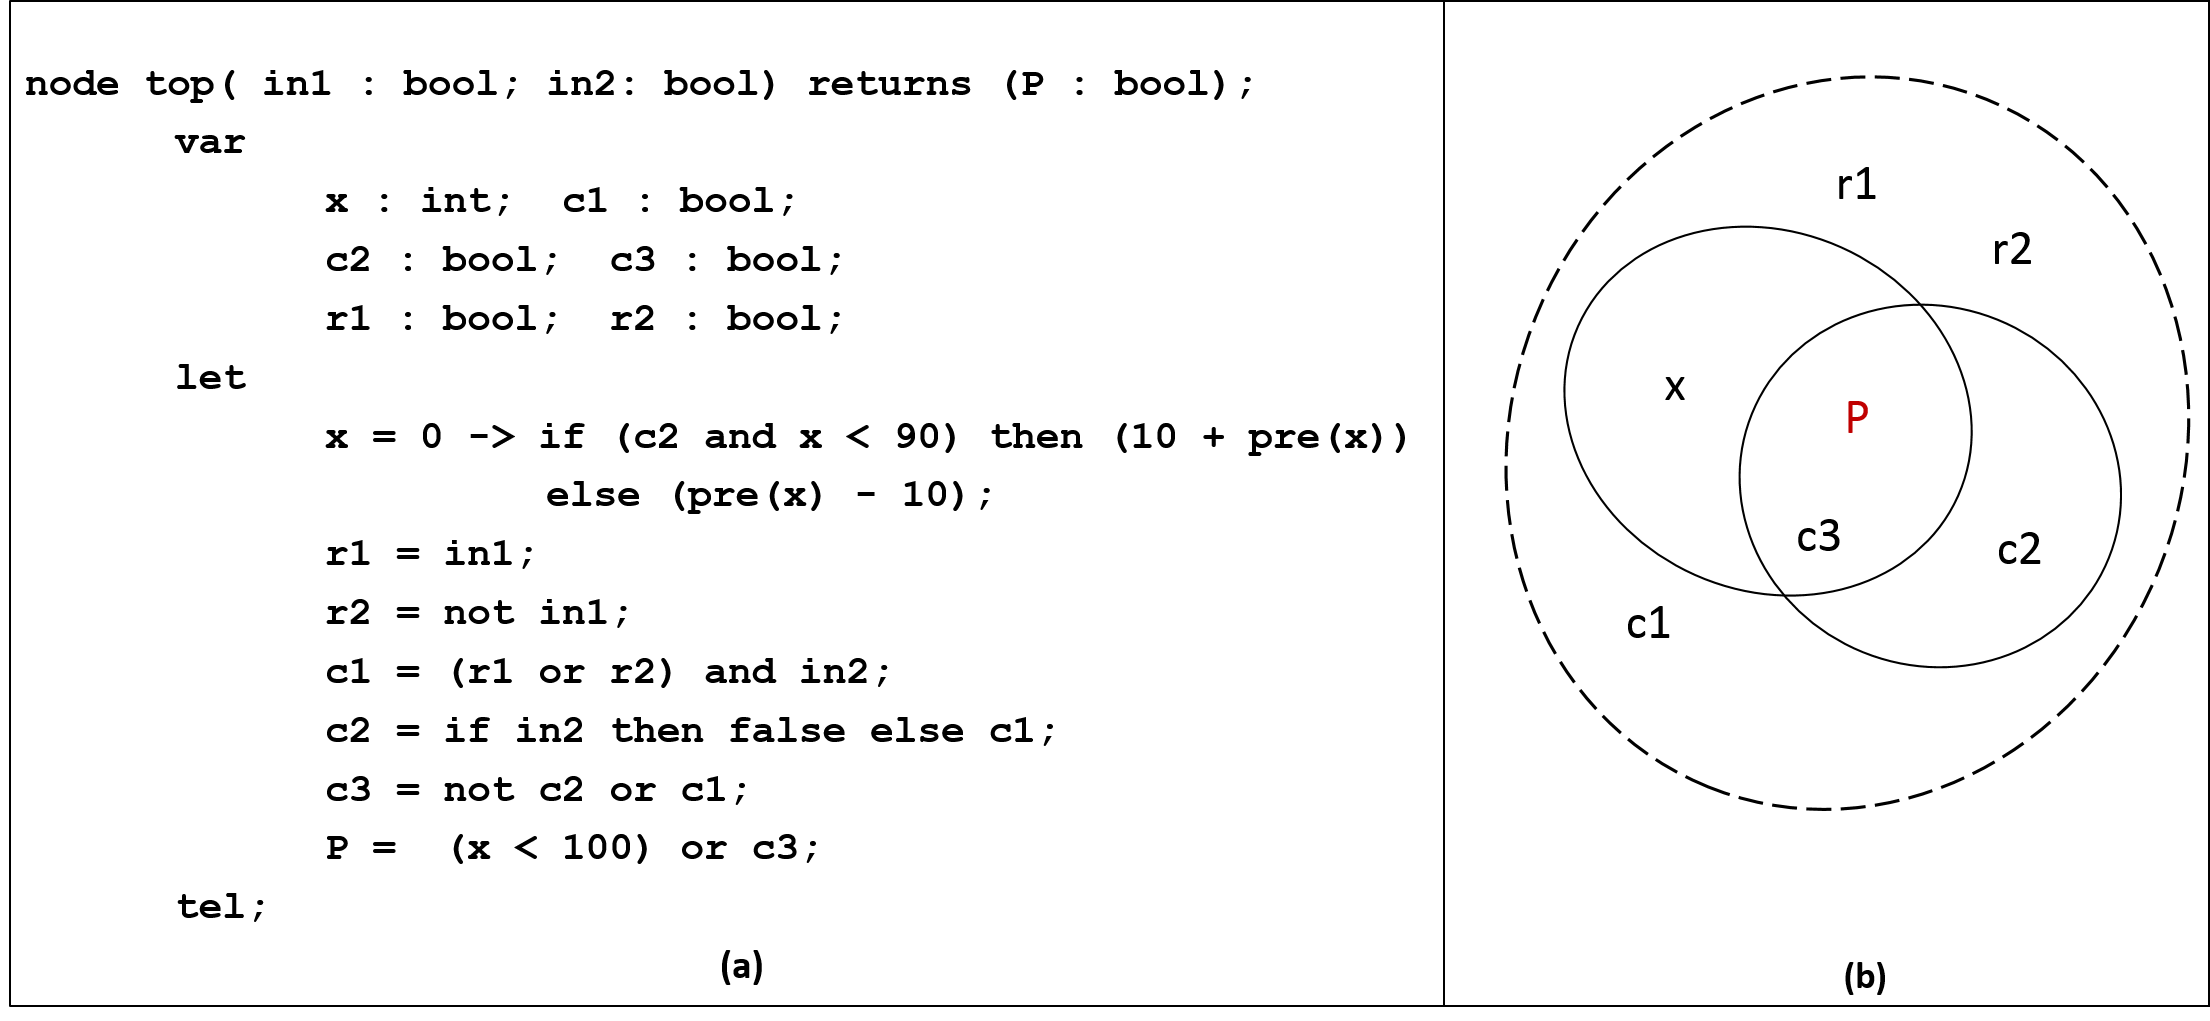
\includegraphics[width=0.8\textwidth]{figs/ex.png}
%\vspace{-0.1in}
%\caption{A Lustre model with property $P$}
%\label{fig:ex}
%\end{center}
%\end{figure*}

%% We put the image here so it shows up side-by-side with fig:ex-after
\begin{figure}[t]
\centering
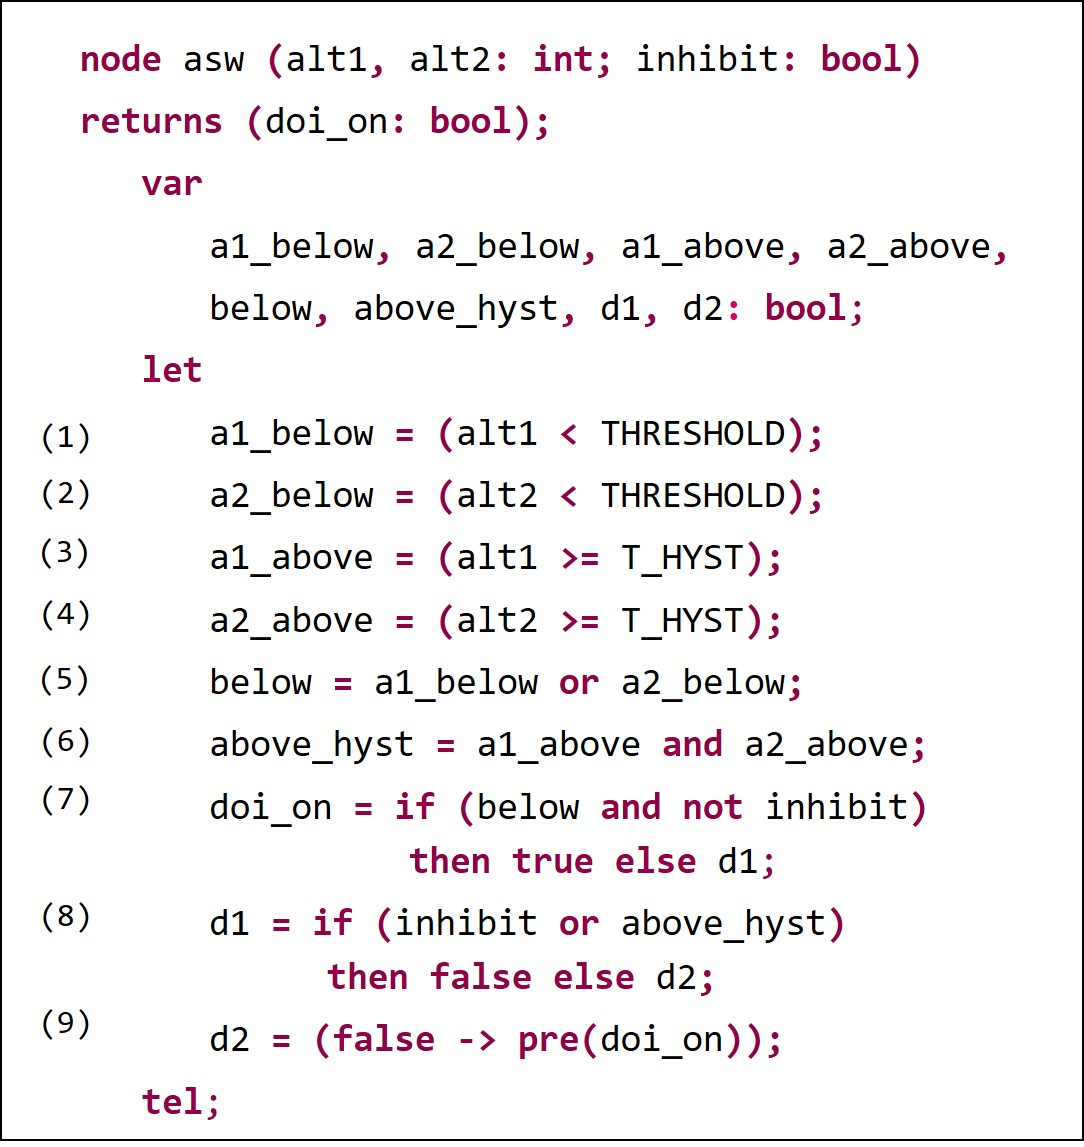
\includegraphics[width=0.9\columnwidth]{figs/code.jpg}
%{\smaller
%\begin{verbatim}
%node asw(alt1, alt2: int; inhibit: bool)
%        returns (doi_on: bool);
%var
%   a1_below, a2_below, a1_above, a2_above,
%   below, above_hyst, d1, d2: bool;
%let
%   a1_below = (alt1 < THRESHOLD);        // (1)
%   a2_below = (alt2 < THRESHOLD);        // (2)
%   a1_above = (alt1 >= T_HYST);          // (3)
%   a2_above = (alt2 >= T_HYST);          // (4)
%   below = a1_below or a2_below;         // (5)
%   above_hyst = a1_above and a2_above;   // (6)
%   doi_on = if (below and not inhibit)   // (7)
%        then true else d1;
%   d1 = if (inhibit or above_hyst)       // (8)
%         then false else d2;
%   d2 = (false -> pre(doi_on));          // (9)
%tel;
%\end{verbatim}
%}
\vspace{-0.1in}
\caption{Altitude Switch Model}
\vspace{-0.27in}
\label{fig:asw}
\end{figure}

We will use a very simple system from the avionics domain to illustrate our approach. An Altitude Switch (ASW) is a hypothetical device that turns power on to another subsystem, the Device of Interest (DOI), when the aircraft descends below a threshold altitude and turns the power off again after we ascend over the threshold plus some hysteresis factor.  An implementation of an ASW containing two altimeters written in the Lustre language (simplified and adapted from~\cite{HCW02:ase-deviation}) is shown in Figure~\ref{fig:asw}.  If the system is not ``inhibited'' by the user and either altimeter is below the constant THRESHOLD, then it turns on the DOI; else, if the system is inhibited or both altimeters are above the threshold plus the hysteresis factor (THRESHOLD + HYST), then the DOI is turned off, and if neither condition holds, then in the initial computation it is false and thereafter retains its previous value.  The notation \texttt{(false -> pre(doi\_on))} in equation (9) describes an initialized register in Lustre: in the initial state, the expression is \texttt{false}, and thereafter it is the previous value of \texttt{doi\_on}.  In the remainder of the paper, we will use this model to illustrate aspects of requirements completeness.  %Section \ref{sec:illust}.


\iffalse
\mike{replace with altitude switch example!}

We will use the model in Figure~\ref{fig:ex} (a) as
a running example throughout the paper. This model is written in Lustre~\cite{Halbwachs91:lustre}, which is a synchronous dataflow language used as an input language for various model checkers. For our purposes, a Lustre program
consists of 1) input variables, {\tt in1} and {\tt in2} in the example, 2) output
variables, {\tt P} in the example, and 3) an
equation for each output variable. A Lustre program runs over discrete
time steps. On each step, the input variables take on some values and
are used to compute values for the output variables on the same step.
In addition, equations may refer to the previous value of a variable
using the {\tt pre} operator, like {\tt x} in the example. This operator is underspecified in the
first step, so the arrow operator, {\tt ->}, is used to guard the
{\tt pre} operator. In the first step the expression {\tt e1 -> e2}
evaluates to {\tt e1}, and it evaluates to {\tt e2} in all other steps. We interpret a Lustre program as a model specification by considering
the behavior of the program under all possible input traces. Safety
properties over Lustre can then be expressed as Boolean expressions in
Lustre. A safety property holds if the corresponding expression is
always true for all input traces. For example, the property for
Figure~\ref{fig:ex} is {\tt P}, which is a valid property.

In the example, the structure of the model allows property {\tt P} to be proved in two ways.
Note that {\tt c1}, {\tt r1}, and {\tt r2} do not affect the validity of {\tt P}, which means
if we remove these equations making {\tt c1}, {\tt r1}, and {\tt r2} input, still {\tt P} will be valid.
In other words, no matter what value these equations have, any change in their value is not observable in the value of {\tt P}.
However, we always need equation {\tt c3} to prove {\tt P}. In addition to {\tt c3}, in order for {\tt P} to be valid either {\tt c2} or {\tt x} is required.

In the rest of the paper, we will refer to this example while explaining different coverage notions.
\fi

%% \begin{itemize}
%%     \item Not sure if this should go before or after the background section with a description of Lustre.
%%     \item Need a small but interesting example.  Andrew, do any of the models that you use as jkind tests
%%         function in this way?  It would be nice to look at what we have lying around; we need something
%%         that requires invariants.
%%     \item It would also be good to have a few points of interest with the model-requirement pairing:
%%     \item \quad   vacuity due to an overconstrained environment
%%     \item \quad   definitions within the model that are irrelevant to the proof.
%%     \item Explain the model and the proof process.
%% \end{itemize}

%%  LocalWords:  IVC


\section{Preliminaries}
\label{sec:background}

\newcommand{\ivc}{\textit{IVC}}
\newcommand{\mivc}{\textit{MIVC}}
\newcommand{\bool}[0]{\mathit{bool}}
\newcommand{\reach}[0]{\mathit{R}}
\newcommand{\ite}[3]{\mathit{if}\ {#1}\ \mathit{then}\ {#2}\ \mathit{else}\ {#3}}

%\subsection{Transition Systems and Safety Properties}
Given a state space $U$, a transition system $(I,T)$ consists of an
initial state predicate $I : U \to \bool$ and a transition step
predicate $T : U \times U \to \bool$.
We define the notion of
reachability for $(I, T)$ as the smallest predicate $\reach : U \to
\bool$ which satisfies the following formulas:
\begin{gather*}
  \forall u.~ I(u) \Rightarrow \reach(u) \\
  \forall u, u'.~ \reach(u) \land T(u, u') \Rightarrow \reach(u')
\end{gather*}
A safety property $P : U \to \bool$ is a state predicate. A safety
property $P$ holds on a transition system $(I, T)$ if it holds on all
reachable states, i.e., $\forall u.~ \reach(u) \Rightarrow P(u)$,
written as $\reach \Rightarrow P$ for short. When this is the case, we
write $(I, T)\vdash P$. We assume the transition relation has the structure of a top-level conjunction.  Given $T(u, u') = T_1(u, u') \land \cdots \land T_n(u, u')$ we will write $T = \bigwedge_{i=1..n}T_i$ for short.
By further abuse of notation,
$T$ is identified with the set of its top-level conjuncts. Thus, $T_i \in
T$ means that $T_i$ is a top-level conjunct of $T$, and $S
\subseteq T$ means all top-level conjuncts of $S$ are top-level
conjuncts of $T$. When a top-level conjunct $T_i$ is removed from $T$, it is written as $T \setminus \{T_i\}$. Such a transition system can easily encode our example model in Section~\ref{sec:example}, where each equation defines a conjunct within $T$ that we will denote by the variable assigned; so, $T = \{$ {\small \texttt{a1\_below, a2\_below, a1\_above, a2\_above, one\_below, both\_above, doi\_on, on\_p}} $\}$.

The idea behind finding an IVC for a given property $P$ \cite{Ghass16} is based on inductive proof methods used in SMT-based model checking, such as $K$-induction and IC3/PDR \cite{NFM2012:KaGaTiWh, amla2005analysis, Een2011:PDR}. Generally, an IVC computation technique aims to determine, for any subset $S \subseteq T$, whether $P$ is provable by $S$. Then, a minimal subset that satisfies $P$ is seen as a minimal proof explanation called a minimal Inductive Validity Core.

\begin{definition}{\emph{Inductive Validity Core (\ivc)\cite{Ghass16}:}}
  \label{def:ivc}
  $S \subseteq T$ for $(I, T)\vdash P$ is an Inductive Validity Core,
  denoted by $\ivc(P, S)$, iff $(I, S) \vdash P $.
\end{definition}

\begin{definition}{\emph{Minimal Inductive Validity Core (\mivc) \cite{Ghass16}:}}
  \label{def:minimal-ivc}
  $S \subseteq T$ is a minimal Inductive Validity Core,
  denoted by $\mivc(P, S)$, iff ~$\ivc(P, S) \wedge \forall T_i \in S.~ (I, S\setminus\{ T_i \}) \nvdash P$.
\end{definition}


Note that, given $(I, T) \vdash P$, $P$ always has at least one \mivc, and it may also have many distinct \mivc s corresponding to different proof paths. To capture the latter, the \emph{all \mivc s ($AIVC$)} relation has been introduced in \cite{Murugesan16:renext}.
\begin{definition}{\emph{All \mivc s ($AIVC$):}}
    \label{def:allivcs}
    Given $(I, T) \vdash P$, $AIVC(P)$ is an association to all \mivc s for $P$:
    $$ AIVC(P) \equiv  \{\ S~|~S \subseteq T \land  MIVC(P, S)\} $$
\end{definition}

Fig.~\ref{fig:ivcs} illustrates these notions by a graphical representation of IVCs for property $P = ({\small{\texttt{on\_p}}})$ in the example presented in Section~\ref{sec:example}. As shown in the picture, this property has two distinct \mivc s, which means the model satisfies $P$ in two different ways:  {\small \texttt{\{\{a1\_below, one\_below, doi\_on, on\_p\}, \{a2\_below, one\_below, doi\_on, on\_p\}\}}}, This is because in the implementation, the DOI is turned on when either of the altimeters is below the threshold, while our property states that they both must be below.
Note that there is a subset of model elements, $\{{\small \texttt{a1\_above, a2\_above, both\_above}}\}$, that does not show up in $AIVC(P)$. Elements in such a subset
do not affect the satisfaction of $P$.  In the complete ASW model in~\cite{HCW02:ase-deviation} there are additional properties that use these elements, but they are not necessary for the discussion in this paper.

%As you can see, distinct IVCs may have common elements.
%The intersection of all \mivc s is called the \emph{must} set for $P$.
%And, the other elements constitute a \emph{may} set for $P$ \cite{Murugesan16:renext}:
%\begin{itemize}
%  \item   $MUST (P) = \bigcap AIVC(P)$
%  \item  $MAY(P) = (\bigcup AIVC (P)) \setminus MUST(P)$
%  \item $IRR(P) = T \setminus (\bigcup AIVC(P))$
%\end{itemize}
%\noindent Given property $P$, functions $MUST$, $MAY$, and $IRR$ partition top-level conjuncts of $T$ (model elements) into three disjoint sets \emph{must}, \emph{may}, and \emph{irrelevant}, respectively. $IRR(P)$ returns portion of the model irrelevant to the satisfaction of $P$, which in our running example is $\varnothing$.
%We will make use of this intuition in Section~\ref{subsec:minimality}.

\begin{figure}[t]
 \centering
  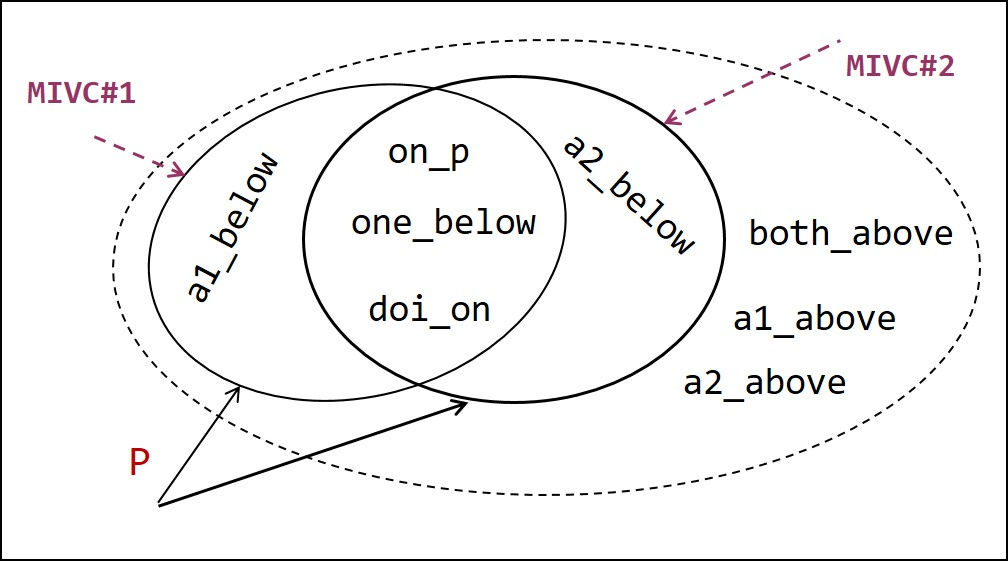
\includegraphics[width=0.8\columnwidth]{figs/ivcs.jpg}
  \vspace{-0.1in}
  \caption{Graphical representation of \mivc s for the model in Fig.~\ref{fig:asw}
  with  $P = ({\small \texttt{on\_p}})$}
  \label{fig:ivcs}
  \vspace{-0.2in}
\end{figure}

%\subsection{Satisfiability}
%In this subsection, we provide a brief background on satisfiability problem.





\section{Inductive Validity Cores}
\label{sec:ivc}

\newcommand{\bq}{\textsc{BaseQuery}\xspace}
\newcommand{\iq}{\textsc{IndQuery}\xspace}
\newcommand{\fq}{\textsc{FullQuery}\xspace}

\newcommand{\mink}{\textsc{MinimizeK}\xspace}
\newcommand{\reduceinv}{\textsc{ReduceInvariants}\xspace}
\newcommand{\minivc}{\textsc{MinimizeIvc}\xspace}

\newcommand{\checksat}{\textsc{CheckSat}\xspace}
\newcommand{\unsatcore}{\textsc{UnsatCore}\xspace}
\newcommand{\unsat}{\textsc{UNSAT}\xspace}
\newcommand{\sat}{\textsc{SAT}\xspace}

Given a transition system which satisfies a safety property $P$, we
want to know which parts of the system are necessary for satisfying
the safety property. One possible way of asking this is, ``What is the
most general version of this transition system that still satisfies
the property?'' The answer is disappointing. The most general system is
$I(s) = P(s)$ and $T(s, s') = P(s')$, i.e., you start in any state
satisfying the property and can transition to any state that still
satisfies the property. This answer gives no insight into the original
system because it has no connection to the original system. In this
section we introduce the notion of {\em inductive validity cores} (IVC) 
which looks at generalizing the original transition system while 
preserving a safety property.

In order to talk about generalizing a transition system, we assume the
transition relation of the system has the structure of a top-level
conjunction. This assumption gives us a structure that we can easily
manipulate as we generalize the system. Given $T(s, s') = T_1(s, s')
\land \cdots \land T_n(s, s')$ we will write $T = T_1 \land \cdots
\land T_n$ for short. By further abuse of notation we will identify
$T$ with the set of its top-level conjuncts. Thus we will write $x \in
T$ to mean that $x$ is a top-level conjuct of $T$. We will write $S
\subseteq T$ to mean that all top-level conjuncts of $S$ are top-level
conjuncts of $T$. We will write $T \setminus \{x\}$ to mean that $T$
with the top-level conjunct $x$ removed. We will use the same notation
when working with sets of invariants.

\begin{definition}{\emph{Inductive Validity Core:}}
  \label{def:ivc}
  Let $(I, T)$ be a transition system and let $P$ be a
  safety property with $(I, T)\vdash P$. We say $S \subseteq
  T$ is a {\em inductive validity core} for $(I, T)\vdash P$ iff $(I,
  S) \vdash P$. When $I$, $T$, and $P$ can be inferred from
  context we will simply say $S$ is an inductive validity core.
\end{definition}

\begin{definition}{\emph{Minimal Inductive Validity Core:}}
  \label{def:minimal-ivc}
  An inductive validity core $S$ for $(I, T)\vdash P$ is minimal iff
  there does not exist $M \subset S$ such that $M$ is an inductive validity core
  for $(I, T)\vdash P$.
\end{definition}

Note that minimal inductive validity cores are not necessarily unique.
For example, take $I = a \land b$, $T = a' \land b'$, and $P = a \lor
b$. Then both $\{a'\}$ and $\{b'\}$ are minimal inductive validity
cores for $(I, T)\vdash P$. However, inductive validity cores do have
the following monotonicity property.

\begin{lemma}
  \label{lem:ivc-monotonic}
  Let $(I, T)$ be a transition system and let $P$ be a safety property
  with $(I, T)\vdash P$. Let $S_1 \subseteq S_2 \subseteq T$. If $S_1$
  is an inductive validity core for $(I, T)\vdash P$ then $S_2$ is an
  inductive validity core for $(I, T)\vdash P$.
\end{lemma}
\begin{proof}
  From $S_1 \subseteq S_2$ we have $S_2 \Rightarrow S_1$. Thus the
  reachable states of $(I, S_2)$ are a subset of the reachable states
  of $(I, S_1)$. \qed
\end{proof}

\begin{algorithm}[t]
  \SetKwInOut{Input}{input}
  \SetKwInOut{Output}{output}
  \Input{$(I, T)\vdash P$}
  \Output{Minimal inductive validity core for $(I, T)\vdash P$}
  \BlankLine
  $S \leftarrow T$ \\
  \For{$x \in S$} {
    \If{$(I, S\setminus\{x\}) \vdash P$}{
      $S \leftarrow S\setminus \{x\}$
    }
  }
  \Return{S}
\caption{Simple algorithm for computing a minimal IVC}
\label{alg:naive}
\end{algorithm}

This lemma gives us a simple, but inefficient algorithm for computing
a minimal inductive validity core, Algorithm~\ref{alg:naive}. The
resulting set of this algorithm is obviously an inductive validity
core for $(I, T)\vdash P$. The following lemma shows that it is also
minimal.

\begin{lemma}
  The result of Algorithm~\ref{alg:naive} is a minimal inductive validity core
  for $(I, T)\vdash P$.
\end{lemma}
\begin{proof}
  Let the result be $R$. Suppose towards contradiction that $R$ is not
  minimal. Then there is an inductive validity core $M$ with $M
  \subset R$. Take $x \in R\setminus M$. Since $x \in R$ it must be
  that during the algorithm $(I, S\setminus\{x\})\vdash P$ is not true
  for some set $S$ where $R \subseteq S$. We have $M \subset R
  \subseteq S$ and $x\not\in M$, thus $M \subseteq S\setminus \{x\}$.
  Since $M$ is an inductive validity core,
  Lemma~\ref{lem:ivc-monotonic} says that $S\setminus \{x\}$ is an
  inductive validity core, and so $(I, S\setminus\{x\})\vdash P$. This
  is a contradiction, thus $R$ must be minimal.
\end{proof}

This algorithm has two problems in practice. First, checking if a
safety property holds is undecidable in general thus the algorithm may
never terminate even when the safety property is easily provable over
the original transition system. Second, this algorithm is very
inefficient since it tries to re-prove the property multiple times.

\begin{algorithm}[t]
  \SetKwInOut{Input}{input}
  \SetKwInOut{Output}{output}
  \Input{$P$ with invariants $Q$ is $k$-inductive for $(I, T)$}
  \Output{Inductive validity core for $(I, T)\vdash P$}
  \BlankLine
  $k \leftarrow \mink(T, P \land Q)$ \\
  $R \leftarrow \reduceinv_k(T, Q, P)$ \\
  \Return{$\minivc_k(I, T, R)$}\\
\caption{Efficient algorithm for computing a nearly minimal inductive validity core}
\label{alg:ivc}
\end{algorithm}

The key to a more efficient algorithm is to make better use of the
information that comes out of model checking. In addition to knowing
that $P$ holds on a system $(I, T)$, suppose we also know something
stronger: $P$ with the invariant set $Q$ is $k$-inductive for $(I,
T)$. This gives us the broad structure of a proof for $P$ which allows
us to reconstruct the proof over a modified transition system.
However, we must be careful since this proof structure may be more
than is actually needed to establish $P$. In particular, $Q$ may
contain unneeded invariants which could cause the inductive validity
core for $P \land Q$ to be larger than the inductive validity core for
$P$. Thus before computing the inductive validity core we first try to
reduce the set of invariants to be as small as possible. This
operation is expensive when $k$ is large so as a first step we
minimize $k$. This is the motivation behind
Algorithm~\ref{alg:ivc}.

\begin{figure}
\begin{align*}
  &\bq_1(I, T, P) \equiv \forall s_0.~ I(s_0) \Rightarrow P(s_0) \\
%%%
  &\bq_{k+1}(I, T, P) \equiv \bq_k(I, T, P) \land~ \\
%
  &\hspace{10pt}\left(\forall s_0, \ldots, s_k.~ I(s_0) \land T(s_0,
  s_1) \land \cdots \land T(s_{k-1}, s_k) \Rightarrow P(s_k)\right)
  \\[5pt]
%%%
  &\iq_k(T, Q, P) \equiv (\forall s_0, \ldots, s_k.~\\
%
  &\hspace{10pt} Q(s_0) \land T(s_0,
  s_1) \land \cdots \land Q(s_{k-1}) \land T(s_{k-1}, s_k) \Rightarrow
  P(s_k)) \\[5pt]
%%%
  &\fq_k(I, T, P) \equiv \\
%
  &\hspace{10pt}\bq_k(I, T, P) \land \iq_k(T, P, P)
\end{align*}
\caption{$k$-induction queries}
\label{fig:queries}
\end{figure}

To describe the details of Algorithm~\ref{alg:ivc} we define queries
for the base and inductive steps of $k$-induction
(Figure~\ref{fig:queries}). Note, in $\iq(T, Q, P)$ we separate the
assumptions made on each step, $Q$, from the property we try to show
on the last step, $P$. We use this separation when reducing the set of
invariants.

We assume that our queries are checked by an SMT solver. That is, we
assume we have a function $\checksat(F)$ which determines if $F$, an
existentially quantified formula, is satisfiable or not. In order to
efficiently manipulate our queries, we assume the ability to create
{\em activation literals} which are simply distinguished Boolean
variables. The call $\checksat(A, F)$ holds the activation literals in
$A$ true while checking $F$. When $F$ is unsatisfiable, we assume we
have a function $\unsatcore()$ which returns a minimal subset of the
activation literals such that the formula is unsatisfiable with those
activation literals held true. In practice, SMT solvers often return a
non-minimal set, but we can minimize the set via repeated calls to
\checksat.

\begin{algorithm}[t]
  $k' \leftarrow 1$ \\
  \While{$\checksat(\neg\iq_{k'}(T, P, P)) = \sat$} {
    $k' \leftarrow k' + 1$ \\
    }
  \Return{$k'$} \\
\caption{$\mink(T, P)$}
\label{alg:minimize-k}
\end{algorithm}

The function $\mink(T, P)$ is defined in
Algorithm~\ref{alg:minimize-k}. This function assumes that $P$ is
$k$-inductive for $(I, T)$. It returns the smallest $k'$ such that $P$
is $k'$-inductive for $(I, T)$. We start checking at $k' = 1$ since
smaller values of $k'$ are much quicker to check than larger ones. The
checking must eventually terminate since $P$ is $k$-inductive. We also
only check the inductive query since we know the base query will be
true for all $k' \leq k$. Although we describe each query in
Algorithm~\ref{alg:minimize-k} separately, in practice they can be
done incrementally to improve efficiency.

\begin{algorithm}[t]
  $R \leftarrow \{P\}$ \\
  Create activation literals $A = \{a_1, \ldots, a_n\}$ \\
  $C \leftarrow \{a_1 \Rightarrow Q_1, \ldots, a_n \Rightarrow Q_n\}$ \\
  \While{$true$} {
    $\checksat(A, \neg\iq_k(T, C, R))$ \\
    \If{$\unsatcore() = \emptyset$}{
      \Return{R}
    }
    \For{$a_i \in \unsatcore()$}{
      $R \leftarrow R \cup \{Q_i\}$ \\
      $C \leftarrow C \setminus \{a_i \Rightarrow Q_i\}$ \\
    }
  }
\caption{$\reduceinv_k(T, \{Q_1, \ldots, Q_n\}, P)$}
\label{alg:reduce-invariants}
\end{algorithm}

The function $\reduceinv_k(T, \{Q_1, \ldots, Q_n\}, P)$ is defined in
Algorithm~\ref{alg:reduce-invariants}. This function assumes that $P
\land Q_1 \land \cdots \land Q_n$ is $k$-inductive for $(I, T)$. It
returns a set $R \subseteq \{P, Q_1, \ldots, Q_n\}$ such that $R$ is
$k$-inductive for $(I, T)$. Like \mink, this function only checks the
inductive query since each element of $R$ is an invariant and
therefore will always pass the base query. A significant complication
for reducing invariants is that some invariants may mutually need each
other, even though none of them is needed to prove $P$. Thus in
Algorithm~\ref{alg:reduce-invariants} we find a minimal set of
invariants needed to prove $P$, then we find a minimal set of
invariants to prove those invariants, and so on. We terminate when no
more invariants are needed to prove the properties in $R$.

This iterative lemma determination does not guarantee a minimal
result. For example, we may find $P$ requires just $Q_1$, that $Q_1$
requires just $Q_2$, and that $Q_2$ does not require any other
invariants. This gives the result $\{P, Q_1, Q_2\}$, but it may be
that $Q_2$ alone is enough to prove $P$ thus the original result is
not minimal. Also note, we do not care about the result of \checksat,
only the \unsatcore that comes out of it. Since $P \land Q_1 \land
\cdots \land Q_n$ is $k$-inductive, we know the \checksat call will
always return \unsat.

\mike{I think we want to be slightly more formal in our reasoning
  about these algorithms, defining soundness (and when possible,
  minimality) lemmas for each.}
\andrew{I'm happy with the level of detail, but I'm fine if we add
  more. If you want to sketch out the outline of what you are
  thinking, I'm happy to fill in the details.}

\begin{algorithm}[t]
  Create activation literals $A = \{a_1, \ldots, a_n\}$ \\
  $T \leftarrow (a_1 \Rightarrow T_1) \land \cdots \land (a_n \Rightarrow T_n)$ \\
  $\checksat(A, \neg\fq_k(I, T, P))$ \\
  $R \leftarrow \emptyset$ \\
  \For{$a_i \in \unsatcore()$}{
    $R \leftarrow R \cup \{T_i\}$
  }
  \Return{R}
\caption{$\minivc_k(I, \{T_1, \ldots, T_n\}, P)$}
\label{alg:minimize-ivc}
\end{algorithm}

The function $\minivc_k(I, \{T_1, \ldots, T_n\}, P)$ is defined in
Algorithm~\ref{alg:minimize-ivc}. This function assumes that $P$ is
$k$-inductive for $(I, T)$. It returns a minimal inductive validity
core $R \subseteq \{T_1, \ldots, T_n\}$ such that $P$ is $k$-inductive
for $(I, R)$.

Our full inductive validity core algorithm in Algorithm~\ref{alg:ivc}
does not guarantee a minimal inductive validity core. One reason is
that \reduceinv does not guarantee a minimal set of invariants. A
larger reason is that we only consider the invariants that the
algorithm is given at the outset. It is possible that there are other
invariants which could lead to a smaller inductive validity core, but
we do not search for them. In Section~\ref{sec:exprm}, we show that in
practice our algorithm is nearly minimal and much more efficient that
the naive algorithm.

\andrew{We should find a way to clean the following argument. I'm not
  sure if it can be simplified, but perhaps we can present it better.}

In general, determining if an inductive validity core is minimal is as
hard the underlying model checking. Given a model checking question
$(I, T)\vdash^? P$ consider adding fresh varaibles $e_1$ and $e_2$ to
obtain a system with initial state predicate $I \land e_1 \land e_2$
and transition predicate $(T \land (\neg P' \Rightarrow e_1')) \land
(e_1' \Rightarrow e_2')$. This extended system has the property $P
\lor e_2$. Thus $S = \{T \land (\neg P' \Rightarrow e_1'), e_1'
\Rightarrow e_2'\}$ is an inductive validity core. Unless $P$ is a
tautology, $\{e_1' \Rightarrow e_2'\}$ will not be an inductive
validity core. The set $\{T \land (\neg P' \Rightarrow e_1')\}$ will
be an inductive validity core if and only if $(I, T)\vdash P$. Thus
decidability of minimality for inductive validity cores is as hard as
model checking.

%%% Local Variables:
%%% mode: latex
%%% TeX-master: "main.tex"
%%% End

%%  LocalWords:  Lustre iff TODO invariants Minimality BaseQuery
%%  LocalWords:  InductiveQuery FullQuery MinimizeK ReduceInvariants
%%  LocalWords:  MinimizeIVC CheckSat UnsatCore UNSAT


\section{Implementation}
\label{sec:impl}

We have implemented the inductive validity core algorithms in the
previous section in two tools: {\em JKind}, which performs the \ucalg
algorithm, and {\em JSupport}, which can compute either the \bfalg or
the \ucbfalg algorithm (using JKind as a subprocess). Moreover, our
implementation of \ucbfalg uses an additional feature of JKind to
store and re-use discovered invariants between separate runs. This
reduces some of the cost of attempting to re-prove a property multiple
times. These tools operate over the Lustre
language~\cite{Halbwachs91:lustre}, which we briefly illustrate below.

\subsection{Lustre and IVCs}

Lustre~\cite{Halbwachs91:lustre} is a synchronous dataflow language
used as an input language for various model checkers. The textual
models in Figures~\ref{fig:ex-before} and \ref{fig:ex-after} are
written in Lustre. We will use model in Figure~\ref{fig:ex-before} as
a running example in this section. For our purposes, a Lustre program
consists of 1) input variables, {\tt x} in the example, 2) output
variables, {\tt a}, {\tt b}, and {\tt y} in the example, and 3) an
equation for each output variable. A Lustre program runs over discrete
time steps. On each step, the input variables take on some values and
are used to compute values for the output variables on the same step.
In addition, equations may refer to the previous value of a variable
using the {\tt pre} operator. This operator is underspecified in the
initial step, so the arrow operator, {\tt ->}, is used to guard the
{\tt pre} operator. In the initial step the expression {\tt e1 -> e2}
evalutes to {\tt e1}, and it evaluates to {\tt e2} in all other steps.

We interpret a Lustre program as a model specification by considering
the behavior of the program under all possible input traces. Safety
properties over Lustre can then be expressed as Boolean expressions in
Lustre. A safety property holds if the corresponding expression is
always true for all input traces. For example, the property for
Figure~\ref{fig:ex-before} is {\tt y >= 0}, which is a valid property.

It is straightforward to translate this interpretation of Lustre into
the traditional initial and transition relations. We will show this by
continuing with the example in Figure~\ref{fig:ex-before}. First we
introduce a new Boolean variable $init$ into the state space to denote
when the system is in its initial step. Then we define,
\begin{align*}
  &I((x, a, b, y, \mathit{init})) = \mathit{init} \\
  &T((x, a, b, y, \mathit{init}), (x', a', b', y', \mathit{init'})) = \\
  &\hspace{1.5cm} (a' = f(x', \ite{init}{0}{y})) \land~ \\
  &\hspace{1.5cm} (b' = \ite{a' \geq 0}{a'}{-a'}) \land~ \\
  &\hspace{1.5cm} (y' = b' + (\ite{init}{0}{y})) \land ~\\
  &\hspace{1.5cm} \neg\mathit{init'}
\end{align*}
A safety property such as {\tt y >= 0} is translated into
$\mathit{init} \lor (y \geq 0)$. Nested uses of arrow and pre
operators are handled by introducing new output variables for nested
expressions, though such details are unimportant for our purposes.

Each equation in the Lustre program is translated into a single
top-level conjunct in the transition relation. This is very convenient
as the IVC of a Lustre property can be reported in terms of the output
variables whose equations are part of the IVC. Equivalently, the
interpretation of an IVC for a Lustre property is that any output
variable that is not part of the IVC can be turned into an input
variable, its equation thrown away, while preserving the validity of
the property.

\subsection{JKind}

JKind is an infinite-state model checker for safety properties. JKind
proves safety properties using multiple cooperative engines in
parallel including $k$-induction, property directed reachability, and
template-based lemma generation. JKind accepts Lustre programs written
over the theory of linear integer and real arithmetic. In the back-end,
JKind uses an SMT-solver such as Yices, Z3, CVC4, MathSAT, or
SMTInterpol.

JKind works on multiple properties simulatenously. When a property is
proven and IVC generation is enabled, an additional parallel engine
executes Algorithm~\ref{alg:ivc} to generate a near-minimal IVC.

JKind accepts an annotation on its input Lustre program indicating
which outputs variables to consider for IVC generation. Output
variables not mentioned in the annotation are implicitly included in
all IVCs. This allows the implementation focus on the variables
important to the user and ignore, for example, administrative
equations. This is even more important for tools which generate Lustre
as they often create many such administrative equations which simply
wire together more interesting expressions.


%\subsection{Experiment}
%\label{sec:experiment}

\newcommand{\takeaway}[1]{
\vspace{6pt}
\noindent\fbox{\parbox{0.975\columnwidth}{#1}}
\vspace{6pt}
}
 the overhead
in discovering all IVCs is a linear in the number of unique IVC
in the problem multiplied by the cost for finding a proof for
%\mike{What do we want to call our efficient algorithm: IVC?}

%We would like to investigate both the {\em efficiency} and {\em
%  minimality} of our three algorithms: the naive brute-force
%algorithm (\bfalg), the UNSAT core-based algorithm (\ucalg), and the
%combined UNSAT core followed by brute-force minimization algorithm
%(\ucbfalg). Efficiency is computed in terms of wall-clock time: how
%much overhead does the IVC algorithm introduce? Minimality is
%determined by the size of the IVC: cores with a smaller number of
%variables are preferred to cores with a larger number of variables.
%Finally, we are interested in the {\em diversity} of solutions: how
%often do different tools/algorithms generate different minimal IVCs?
%
%The use of \texttt{JKind} allows additional dimensions to our investigation: it supports two different inductive algorithms: $k$-induction and PDR, and a ``fastest'' mode, that runs both algorithms in parallel.  In addition, \texttt{JKind} supports multiple back-end SMT solvers including Z3~\cite{DeMoura08:z3}, Yices~\cite{Dutertre06:yices}, MathSAT~\cite{Cimatti2013:MathSAT}, and SMTInterpol~\cite{Christ2012:SMTInterpol}.  We would like to determine whether the choice of inductive algorithm affects the size of the IVC, whether different solvers are more or less efficient at producing IVCs, and whether running different solvers/algorithms leads to {\em diversity} of IVC solutions.
%
%Therefore, we investigate the following research questions:
%\begin{itemize}
%    \item \textbf{RQ1:} How expensive is it to compute inductive validity cores using the \bfalg, \ucalg, and \ucbfalg algorithms?
%    \item \textbf{RQ2:} How close to minimal are the IVC sets computed by \ucalg as opposed to the (guaranteed minimal) \ucbfalg?  How do the sizes of IVCs compare to static slices of the model?
%    \item \textbf{RQ3:} How much {\em diversity} exists in the solutions produced by different solver/induction algorithm configurations?
%\end{itemize}
%
%\subsection{Experimental Setup}
%In this study, we started from a suite of 700 Lustre models developed
%as a benchmark suite for~\cite{Hagen08:FMCAD}. We augmented this suite
%with 81 additional models from recent verification projects including
%avionics and medical devices~\cite{QFCS15:backes,hilt2013}. Most of
%the benchmark models from~\cite{Hagen08:FMCAD} are small (10kB or less,
%with 6-40 equations) and contain a range of hardware benchmarks and
%software problems involving counters. The additional models are much
%larger: around 80kB with over 300 equations. We added the new
%benchmarks to better check the scalability for the tools, especially
%with respect to the brute force algorithm.
%%
%%\mike{MORE HERE...stats on size, reasons for add'l models.}
%Each benchmark model has a single property to analyze.  For our purposes, we are only interested in models with a {\em valid} property (though it is perhaps worth noting that there is no additional computation---and thus no overhead---using the \texttt{JKind} IVC options for {\em invalid} properties).  In our benchmark set, 295 models yield counterexamples, and 10 additional models are neither provable nor yield counterexamples in our test configuration (see next paragraph for configuration information).  The benchmark suite therefore contains 476 models with valid properties, which we use as our test subjects.
%
%For each test model, we computed \ucalg in 12+1 configurations: the
%twelve configurations were the cross product of all solvers \{Z3,
%Yices, MathSAT, SMTInterpol\} and inductive algorithms
%\{$k$-induction, PDR, fastest\}, and the remaining (+1) configuration
%was an instance of \bfalg run on Yices, which is the default solver in
%\texttt{JKind}. In addition, for each of the 12 configurations, we ran an
%instance of \texttt{JKind} without IVC to examine overhead. The experiments
%were run on an Intel(R) i5-2430M, 2.40GHz, 4GB memory machine, with a
%1 hour timeout for each analysis on any model. The data gathered for
%each configuration of each model included the time required to check
%the model without IVC, with IVC, and also the set of elements in the
%computed IVC.\footnote{The benchmarks, all raw experimental results,
%  and computed data are available on \cite{expr}.}
%
%Note that not all analysis problems were solvable with all algorithms: for all solvers, $k$-induction (without IVC) was unable to solve 172 of the examples.  When comparing minimality of different solving algorithms, we only considered cases where both algorithms provided a solution (as will be discussed in more detail in Section~\ref{sec:minimality}).
%
%\iffalse
%\begin{itemize}
%    \item an algorithm to compute a truly minimal set of support, i.e. \texttt{JSupport}.
%    \item given a LUS model, a static crawler which automatically marks all equations of a node in the initial support set of a property.
%    \item some trackers that measure the verification time with/ without support computation.
%   % \item some minor changes in the XML writers.
%\end{itemize}
%
%\mike{My thoughts on this section: mostly, it needs more structure: more information on the properties of the models: size, provenance, etc., a broken out subsection on the description of the experimental setup, etc}
%
%\mike{I think we want to split out the results in another top-level section}
%
%Experiment:
%\begin{itemize}
%    \item (Overview) describe research questions and goals.
%    \item Experimental setup: tell me about the models: how many, how big are they?  Then, tell me about the experiment: the tool configurations, the machine used for test.
%    \item Data generation: Describe what you measured for each model analysis.
%\end{itemize}
%\fi
%
%
%%%  LocalWords:  minimality ive UNSAT IVC Minimality IVCs PDR Yices
%%%  LocalWords:  MathSAT SMTInterpol RQ JSupport


\section{Results}
\label{sec:results}

\newcommand{\takeaway}[1]{
\vspace{6pt}
\noindent\fbox{\parbox{\columnwidth}{#1}}
\vspace{6pt}
}

In this section, we examine our experimental results from three perspectives: performance, minimality of \ucalg results and diversity.

\iffalse
\mike{Results and Discussion:}
\begin{itemize}
    \item (Overview) Give an overview of results, possibly referencing a graph or two.
    \item Statistical analysis: provide positive and null hypotheses for the research questions.
    \item Evaluation of research questions: statistical results and explanations of the graphs.  One subsection per research question?
    \item Threats to validity: what are our threats?
    Internal validity: not really necessary, I think.
    External validity (how much can the results be generalized):
        1. currently all models are *very small*;
        2. Many programs were drawn from mutations of a relatively small number of ``seed'' programs;
        3. The models are written in Lustre rather than FOL.  This means that the
            top-level conjunctions are all over equations rather than general
            form;
        4. Others?!?
    Construct validity: we are measuring what we think we're measuring: IVC and minimality are reasonably defined.  For discussions of ``completeness'' and ``traceability'' we need to be clear about any claims (probably not in this paper).
\end{itemize}
\fi

\subsection{Performance}
\label{sec:performance}

In this subsection, we examine the performance of our inductive validity core algorithms (research question \textbf{RQ1}).  First we examine the performance overhead of the \ucalg algorithm over the time necessary to find a proof using inductive model checking.  To examine this question, we use the default {\em fastest} option of JKind which terminates when either the k-induction or PDR algorithm finds a proof.  To measure the performance overhead of the \ucalg algorithm, we execute it over the proof generated by the {\em fastest} option.

Since the \ucalg algorithm uses the UNSAT-core facilities of the underlying SMT solver, the performance is dependent on the efficiency of this part of the solver.  Examining Tables~\ref{tab:runtime-ucalg} and~\ref{tab:overhead-ucalg}, it is possible to examine both the aggregate computation time for analysis using the four solvers under evaluation and the overhead imposed by the \ucalg algorithm.  The data suggests that yices (the default solver in JKind) and z3 are the most performant solvers both in terms of computation time and overhead.  Figure~\ref{fig:runtimeall} allows a visualization of the overhead for the \ucalg algorithm running different tools (as well as the \bfalg, discussed below).  For this figure, models are ranked on the x-axis in terms of their analysis time using the z3 solver to perform the proof without performing IVC.

%Figure~\ref{fig:runtimez3} allows a visualization of the overhead for the Z3 solver, where the models are ranked on the x axis in terms of their analysis time without performing \ucalg, and the y-axis describes analysis time with and without \ucalg.

%\mike{Add the raw timings for each solver for proof and proof + \ucalg analysis in Table~\ref{tab:overhead}.}

%Although it is relatively obvious from Table~\ref{tab:overhead}, it is straightforward to demonstrate with statistical significance that Z3 outperforms other solvers.  The hypotheses are as follows: \mike{FILL IN HYPOTHESES}.

%\mike{Do we need hypotheses here?  We could say a 'moderate' performance penalty is under 50\% over the regular solver time}.

\takeaway{The \ucalg algorithm using the Z3 and yices SMT solvers adds a modest performance penalty to the time required for inductive proofs.}

Next, we consider the overhead of \ucalg vs. \bfalg.  Recall from Section~\ref{sec:ivc} that \bfalg requires $n$ model checking runs, where $n$ is the number of conjuncts in the transition relation. As expected, the performance is approximately a linear multiple of the size of the model, so larger models yield substantially lower performance.\footnote{for Lustre models, the number of conjuncts is equivalent to the number of equations in the Lustre model.}  We run the brute-force algorithm using yices as it is the default solver for JKind and is close to z3 in terms of computation time.  For 19 models, \bfalg times out after 1 hour.   Figure~\ref{fig:runtimeall} shows the overhead of \bfalg in comparison to \ucalg with multiple solvers.

\takeaway{The brute-force algorithm \bfalg adds a substantial performance penalty to inductive proofs in all cases and is not scalable enough to compute a minimal core for large analysis problems.}

Finally, we consider the combined \ucbfalg algorithm, in which we first run the \ucalg to determine a close-to-minimal set of support, then run the \bfalg on the remaining set.  The overhead of this algorithm is considered in Tables~\ref{tab:runtime-ucbfalg} and~\ref{tab:overhead-ucbfalg}.  While considerably slower than the \ucalg, this approach can still be used for reasonably sized models.

\begin{figure*}
  \centering
  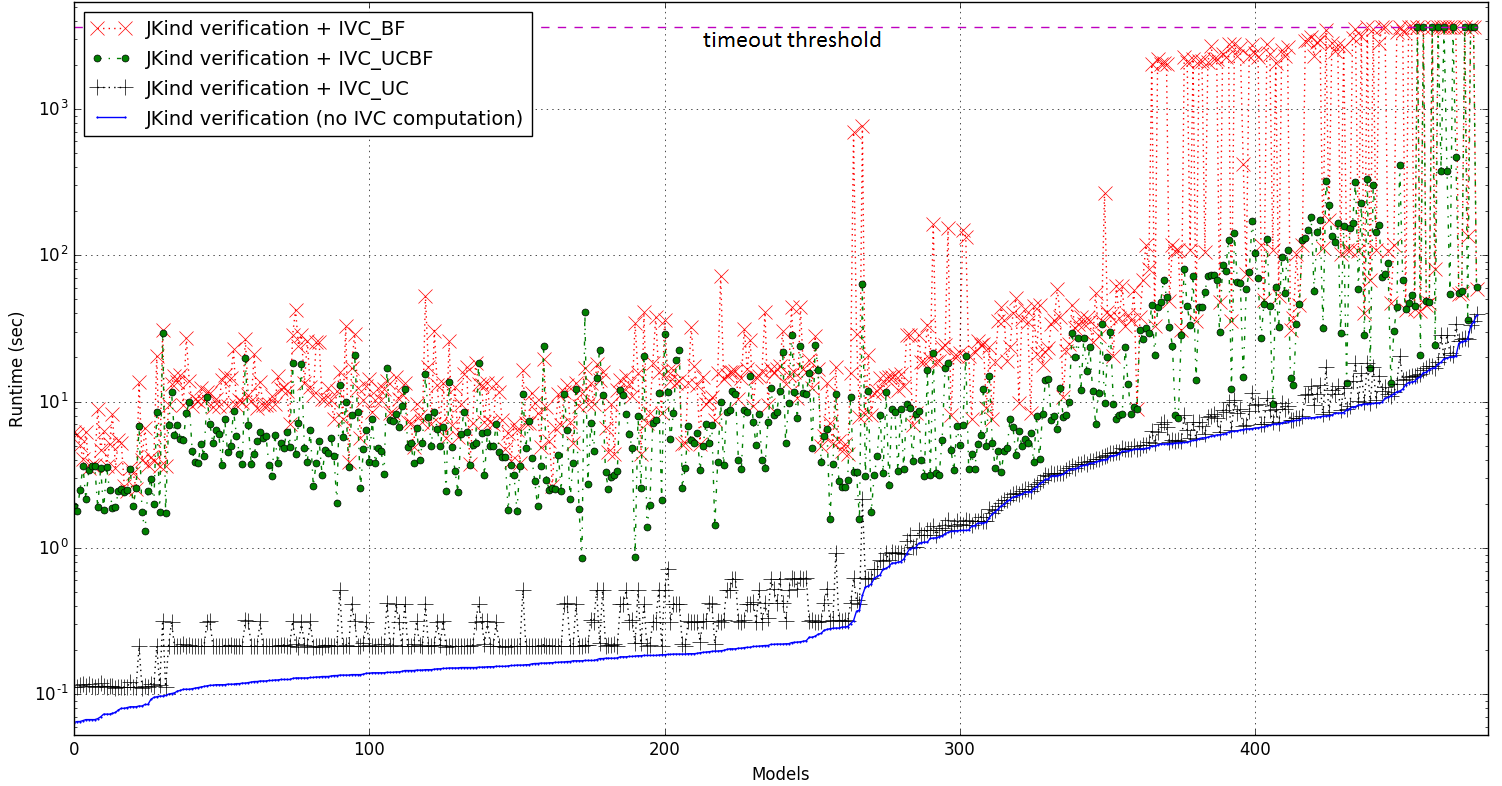
\includegraphics[width=\textwidth]{figs/timing_analyses.png}
  \vspace{-0.3in}
  \caption{Runtime of \bfalg, \ucbfalg, \ucalg algorithms for Yices}\label{fig:runtimeall}
\end{figure*}

%\vspace{-0.5in}
\begin{figure*}
  \centering
  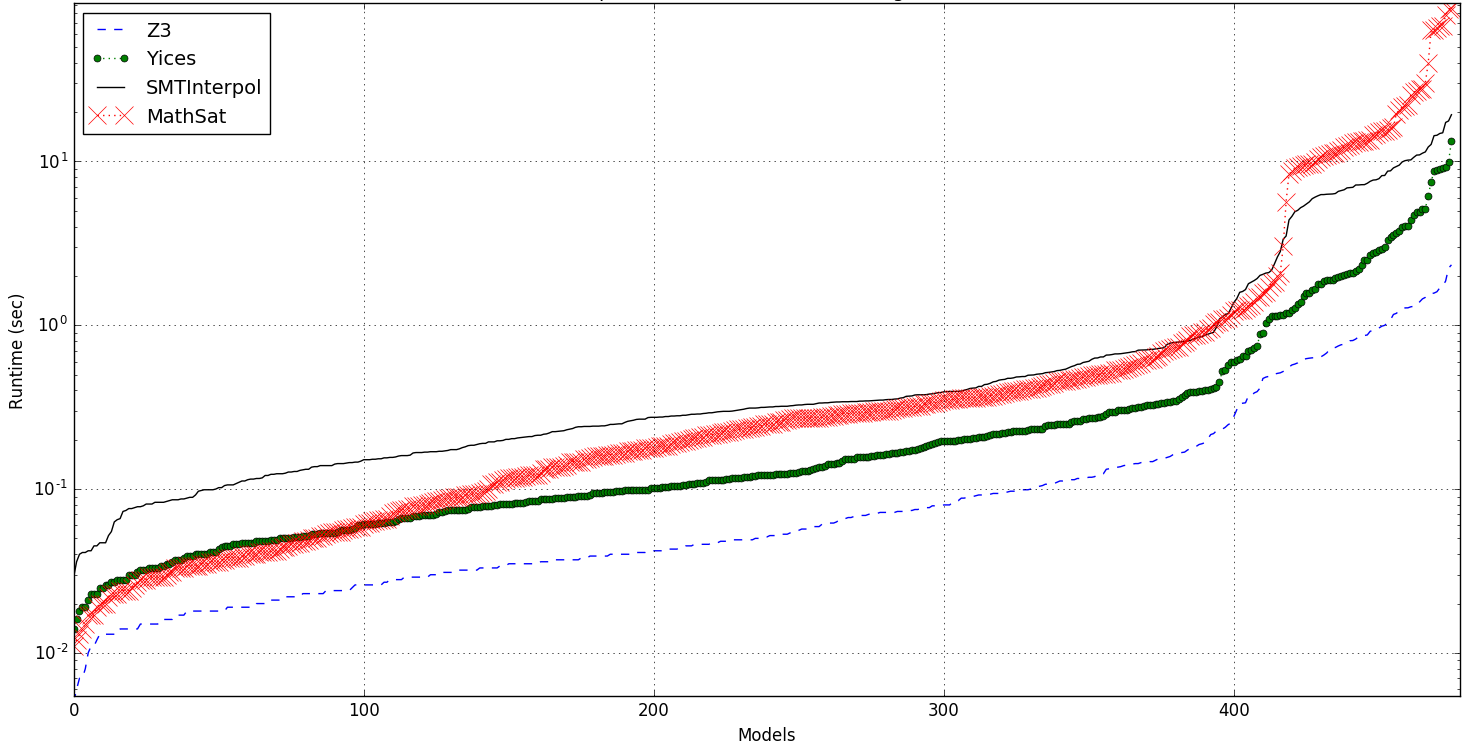
\includegraphics[width=\textwidth]{figs/performance.png}
  \vspace{-0.3in}
  \caption{\ucalg performance on different solvers}\label{fig:performance}
\end{figure*}

\begin{table}
  \centering
  \begin{tabular}{ |c||c|c|c|c| }
    \hline
     runtime (sec) & min & max & mean & stdev \\[0.5ex]
    \hline\hline
 %   JSupport & 2.381 & 165.157 & 21.533 & 23.533 \\[0.5ex]
    Z3   & 0.005 & 2.335 & 0.192 & 0.355 \\[0.5ex]
    Yices &   0.014  & 13.297   & 0.589 & 1.473 \\[0.5ex]
    SMTInterpol& 0.029 & 19.254 &  1.396 & 2.991 \\[0.5ex]
    MathSAT & 0.011 & 86.421 &  3.071 & 10.403 \\[0.5ex]
    \hline
  \end{tabular} \\
  \caption{\ucalg runtime with different solvers}
  \label{tab:runtime-ucalg}
\end{table}

\begin{table}
  \centering
  \begin{tabular}{ |c||c|c|c|c| }
    \hline
     solver & min & max & mean & stdev \\[0.5ex]
    \hline
    Z3   & 0.73\% & 84.13\% & 17.38\% & 16.92\% \\[0.5ex]
    Yices &   0.17\%  & 351.47\%   & 52.20\% & 54.50\% \\[0.5ex]
    SMTInterpol& 1.46\% & 175.75\% &  46.81\% & 37.35\%\\[0.5ex]
    MathSAT & 0.78\% & 955.52\% &  80.21\% & 112.92\%\\[0.5ex]
    \hline
  \end{tabular}
  \caption{Overhead of \ucalg computations using different solvers}
  \label{tab:overhead-ucalg}
\end{table}

\begin{table}
  \centering
  \begin{tabular}{ |c||c|c|c|c| }
    \hline
     runtime (sec) & min & max & mean & stdev \\[0.5ex]
    \hline
    Yices &   0.678  & 3600.0   & 91.594 & 490.008 \\[0.5ex]
    \hline
  \end{tabular}
  \caption{\ucbfalg runtime with Yices}
  \label{tab:runtime-ucbfalg}
\end{table}

\begin{table}
  \centering
  \begin{tabular}{ |c||c|c|c|c| }
    \hline
     solver & min & max & mean & stdev \\[0.5ex]
    \hline
    Yices & 122.50\%  & 30092.78\%   & 3195.90\% & 3896.05\% \\[0.5ex]
    \hline
  \end{tabular}
  \caption{Overhead of \ucbfalg algorithm using Yices}
  \label{tab:overhead-ucbfalg}
\end{table}
% over = in

\begin{table}
  \centering
  \begin{tabular}{ |c|c|c|c| }
    \hline
     solver & PDR & k-induction & \textbf{total} \\
    \hline
      z3 & 2378 & 2379 & 4757 \\
      yices & 2384 & 2376 & 4760 \\
      MathSAT & 2375 & 2369 & 4744 \\
      SMTInterpol & 2378 & 2368 & 4746 \\
    \hline
      \textbf{total} & 9515 & 9492 &   \\
    \hline
  \end{tabular}
  \caption{Aggregate IVC sizes produced by \ucalg\ using different inductive algorithms and solvers}
  \label{tab:minimality-algorithm-solvers}
\end{table}

\begin{table}
  \centering
  \begin{tabular}{ |c||c|c|c|c| }
    \hline
     solver & min & max & mean & stdev \\[0.5ex]
    \hline
    Yices &   0.0\%   & 7.25\% & 0.20\% & 0.50\% \\[0.5ex]
    \hline
  \end{tabular}
  \caption{Increase in IVC Size for \ucalg\ vs. \ucbfalg}
  \label{tab:overhead-ucbfalg}
\end{table}


\begin{figure*}
  \centering
  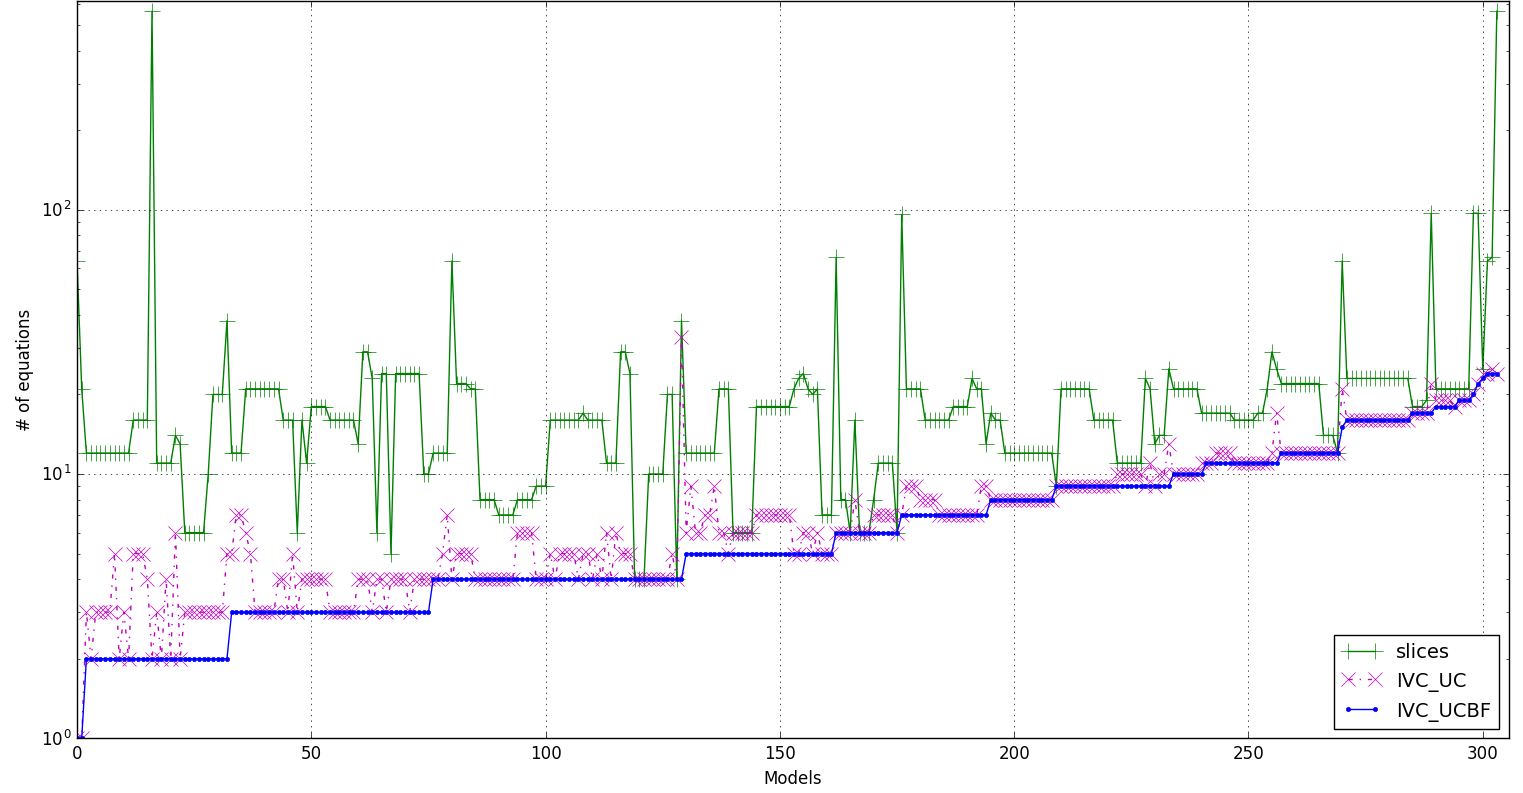
\includegraphics[width=\textwidth]{figs/minimality.png} 
  \caption{IVC sizes produced by \ucalg vs. \ucbfalg for Yices}
  \label{fig:minimality-all}
\end{figure*}

\subsection{Minimality}
\label{sec:minimality}
In this section, we examine the minimality of the cores computed by the \ucalg algorithm using different inductive proof methods and compare it to the cores produced by the combined algorithm (\textbf{RQ2}).  There are three interesting aspects to be examined related to this research question.  First (\textbf{RQ2.1}), does the choice of SMT solver or algorithm used to produce a proof (k-induction or PDR) matter in terms of the minimality of the inductive core?   As mentioned in Section~\ref{sec:ivc}, the \ucalg algorithm is not guaranteed to produce a minimal core due in part to the role of invariants used in producing a proof; as k-induction and PDR use different invariant generation algorithms, it is possible that one or the other is more likely to yield smaller invariant sets.  In addition, differences in the choice of the UNSAT-core algorithms in the different tools could affect the size of the generated core.  However, our algorithm {\em already} does a minimization step.  However,
our algorithm {\em already} does a minimization step on UNSAT-cores,
thus the only differences would be due to one algorithm leading to a
different minimal core than another.

As discussed in Section~\ref{sec:experiment}, k-induction is unable to solve all of the analysis problems; therefore we include only models that are solvable using {\em both} k-induction and PDR by {\em all tools}, 304 models in all.  Examining the aggregate data in Table~\ref{tab:minimality-algorithm-solvers}, we can see the sizes of cores produced by different algorithms and tools.

%if we sum all elements of all cores together, that PDR has an smaller core size in aggregate than k-induction.
%However, the data is noisy, and to examine \textbf{RQ2.1} systematically, we construct a hypothesis that PDR will, in general, equal or outperform k-induction on an arbitrary model:

%\mike{ADD HYPOTHESIS/NULL HYPOTHESIS HERE}

%Although the aggregate data suggests that PDR will yield a smaller core (on average) than k-induction, this claim is not supported for a given model with significance.

\takeaway{Neither PDR nor k-induction yields a smaller inductive validity core in general.}


%we already perform a linear scan of the cores generated by the SMT solver to remove unnecessary conjuncts

The next question (\textbf{RQ2.2}) asks how close to minimal are the cores produced by \ucalg\ vs. the (guaranteed minimal) cores produced by the \ucbfalg\ algorithm?  Note that we cannot measure the distance on all models because the combined algorithm times out on 9 of the larger models.  We therefore examine the distance from minimal cores produced by the combined algorithm for models in which it completes within the one hour timeout.  For comparison, we run the \ucalg\ algorithm in each tool with the default {\em fastest} algorithm, which will use the result of either k-induction or PDR.  A graph showing the size of the IVCs for each model produced by the yices solver is shown in Figure~\ref{fig:minimality-all}.  In the figure, the models are ranked along the x-axis by the size of the core produced by \ucbfalg.  The figure demonstrates that while on average there is a modest change in minimality that there can be substantial variance on the sizes of the cores produced by the \ucalg\ algorithm.

\takeaway{The \ucalg algorithm computes cores that are 0\% to 7.25\% larger than those produced by \ucbfalg, with substantial variance in the results.}


\iffalse
\ela{I think this is not needed: \\In terms of size, we calculated the size of the biggest and smallest sets per model, then added them together for all models. The same calculation has been done for \texttt{JSupport}:
\begin{itemize}
  \item $A\_JS$: the aggregate number of elements in support sets computed by \texttt{JSupport} = 3078
  \item $A\_Ss$: the aggregate number of elements in the \emph{smallest} support sets = 3474;
  this implies $A\_Ss$ is 12\% greater than $A\_JS$.
  \item $A\_Bs$: the aggregate number of elements in the \emph{biggest} support sets = 3586;
  this implies $A\_Bs$ is 16\% greater than $A\_JS$.
\end{itemize}}
Average size of sets computed by \texttt{ReduceSupport} is 8.55. And, average size of sets computed by \texttt{JSupport} is 7.60. Therefore, in average, support sets computed by \texttt{ReduceSupport} are 88\% close to minimal, in terms of their size.  %  (1 - ((8.55 - 7.6)/ 7.6))  * 100 = 87.5%
Since \texttt{JSupport}, with a great percentage, most of the time computed the smallest support set, we compared the size of the sets computed by \texttt{ReduceSupport} with \texttt{JSupport}. For each configuration, we collected the difference between its support size and \texttt{JSupport} per model. Table~\ref{tab:minimality} shows the result of analysis.
\fi

\begin{table}
  \centering
  \begin{tabular}{ |c|c|c|c| }
    \hline
     min & max & mean & stdev \\[0.5ex]
    \hline
    %sample size = 4196
     0.0   & 0.878 & 0.026 & 0.059 \\[0.5ex]
    \hline
  \end{tabular}
  \caption{Pairwise Jaccard distances among all models}
  \label{tab:jaccard-avg}
\end{table}

\begin{figure*}
  \centering
  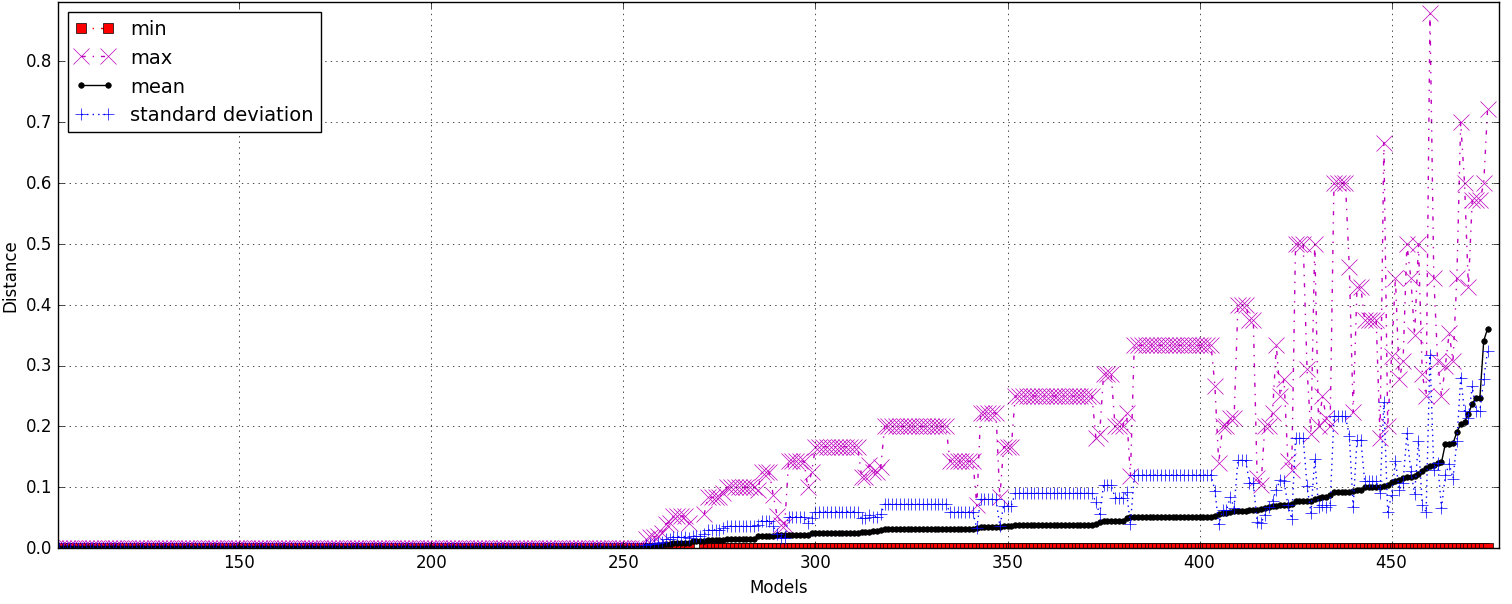
\includegraphics[width=\textwidth]{figs/jacdis2.png} \\
  \caption{Pairwise Jaccard distance between IVCs}\label{fig:jacdis}
\end{figure*}

\subsection{Diversity}
\label{sec:diversity}
Recall from Section~\ref{sec:ivc} that a {\em minimal} core is any core leading to a proof such that if you remove any of the conjuncts from the core, it no longer produces a proof.  For certain models and properties, it is possible that there are many minimal cores that will lead to a proof.  In this section, we examine the issue of diversity: do different tools and algorithms lead to {\em different} minimal cores?  This is both a function of the models and the solution algorithms: for certain models, there is only one possible minimal core, whereas other models might have many. Given that there are multiple solutions, the interesting question is whether using different tools and algorithms will lead to different solutions.  Note that this question is closely tied to that of {\em minimality}, which we examined in the previous section.

Our exploration in this case is not exhaustive, but only exploratory.  The reason it is considered is that it has substantial relevance to some of the uses of the tool: e.g., for constructing traceability matrices from proofs.  Given diversity of results, we may wish to distinguish {\em must} traceability elements from {\em may} traceability elements across a set of diverse solutions, and consider more systematic explorations of diversity in future work.

To measure diversity of IVCs, we use Jaccard distance:
\begin{definition}{\emph{Jaccard distance:}}
  \label{def:dj}
  $d_J(\small{A}, \small{B}) = 1 - \frac{|A \cap B|}{|A \cup B|} ,\\ 0 \leq d_J(\small{A}, \small{B}) \leq 1$
\end{definition}
\noindent Jaccard distance is a standard metric for comparing finite sets (assuming that both sets are non-empty) by comparing the size of the intersection of two sets over its union.  For each model in the benchmark, the experiments generated 13 different sets of support. Therefore, we obtained $\binom{13}{2} = 78$ combinations of pairwise distances per model. Then, minimum, maximum, average, and standard deviation of the distances were calculated (Fig~\ref{fig:jacdis}), by which, again, we calculated these four measures among all models.  As seen in Table~\ref{tab:jaccard-avg}, on average, the Jaccard distance between different solutions is small, but the maximum is close to 1, which indicates that even for our exploratory analysis, there are models for which the tools yield substantially diverse solutions.  The diversity between solutions is represented graphically in Figure~\ref{fig:jacdis}, where for each model, we present the min, max, and mean pairwise distance of the solutions produced by algorithm \ucalg for each model, ranked by the mean distance.

\iffalse
\mike{Do we want the discussion below?  I am not sure that it adds much}

To measure the overall similarity among all sets, instead of a pairwise comparison, we used \emph{frequent pattern mining} \cite{han2007frequent}. To define an overall similarity among all sets of support of a given model\footnote{Note that all models in the benchmarks are single property; hence, instead of saying a set of support of a given \emph{property}, we just refer it as the support set of the \emph{model} while explaining the experimental results.}, we calculated a \emph{core} support set for each model in the benchmark, which can be considered as a closed frequent pattern; a core set of model $M$, denoted by $C_M$, is defined as:
\begin{definition}
  \label{def:core}
  $C_M = \bigcap_{i=1}^{13} s_{Mi},   \hspace{9pt} s_{Mi} \in S_M$
\end{definition}

Based on this notion, overall dissimilarity, denoted by $D_{J\{M\}}$, is defined as follows:

\begin{definition}
  \label{def:dis}
  $D_{J\{M\}} =  \frac{\sum_{i=1}^{12}d_J(s_{Mi}, C_M)}{12},   \hspace{9pt} s_{Mi} \in S_M$
\end{definition}

Since our goal is to measure the diversity or dissimilarity among sets computed by \texttt{ReduceSupport}, in \ref{def:dis}, we exclude the set generated by \texttt{JSupport}. In Fig~\ref{fig:jacdis}, the \emph{overall distance} line shows $D_{J\{M\}}$ per model, which can be analyzed from the following hypotheses:
\begin{itemize}
  \item H0: variety of obtained sets of support is high (average $D_{J\{M\}}$ of 0.2)
  \item H1: variety of obtained sets of support is small (average $D_{J\{M\}}$ less than 0.2)
\end{itemize}
Table~\ref{tab:variety} shows that, with an effect size of 0.79, H0 can be rejected.
\begin{table}
  \centering
  \begin{tabular}{ |c|c|c|c|c|c| }
    \hline
     min & max & mean & stdev & ES & p-value\\[0.5ex]
    \hline
    %sample size = 395
     0.0   & 0.879 & 0.099 & 0.141 & 0.72 & < 0.00001 \\[0.5ex]
    \hline
  \end{tabular}
  \caption{$D_{J\{M\}}$ among all models}
  \label{tab:variety}
\end{table}
\fi
%summarized as follows:
%\begin{itemize}
%  \item minimum $D_{J\{M\}}$ among all models: 0.0
%  \item maximum $D_{J\{M\}}$ among all models: 0.879
%  \item average $D_{J\{M\}}$ among all models: 0.096
%  \item standard deviation of $D_{J\{M\}}$ among all models: 0.132
%\end{itemize}


\subsection{Discussion}

In the previous section, we presented three algorithms for determining inductive validity cores.  The brute-force algorithm is guaranteed minimal, but is often very slow.  The other two algorithms: the UNSAT-core algorithm \ucalg\ and the combined algorithm \ucbfalg, represent interesting trade-offs.  The \ucalg\ algorithm is much faster, but is not guaranteed to be minimal; the result of this algorithm can be further, and often quite quickly, refined by the combined algorithm.  Thus, we can choose to trade off speed for guaranteed minimality using these two algorithms; the combined algorithm can be viewed as a refinement algorithm that we can terminate either at completion or after a fixed time bound.


%One question that arises is: why is the refinement so much quicker than the brute-force approach?  In our preliminary examination, it appears to be because of the actions performed by JKind on the sub-problems.  When the cores produced by \ucalg\ are minimal or close to minimal, it tends to be the case that removing conjuncts from the core leads to short counterexamples.  When performing the brute-force algorithm, removing the irrelevant pieces of the model require repeated proof search.

Although our experiment does not ask statistical questions, it is still worth examining threats towards generalizing our results.  First, are the models and properties that we chose representative?  We started from an existing benchmark from another research group suite to try to assuage this concern, but most of these models were small, so we extended the benchmark suite with 81 of our own models.  It is possible that our additions skew the results, though these models are immediately derived from previously published work and not modified for our analysis here.  Second, our models and tools use the Lustre language, which is equational, rather than conjuncted transition systems; it is possible (though, in our opinion, unlikely) that arbitrary conjuncts rather than equations will yield different performance or minimality characteristics.



\section{Related work}
\label{sec:related}

%\mike{place in related work}
%{\em Mutations and Universal Properties} It is important to note that some mutations {\em reduce} the state space of the system to be explored; in this case, any universal property (such as the safety properties in~\ref{sec:ts}) that was true of the original system must, by definition, be true of the mutated system.  For such mutations, an alternate notion of {\em vacuity coverage}
%\mike{end placement}


%Different notions of coverage have been well defined in software testing. However, in formal verification, it is very complex to define and compute this notion.
%Usually, coverage techniques in the property-based verification try to measure the quality of the specification in regard to the completeness of a set of properties.

Coverage in verification was introduced in \cite{hoskote1999coverage, katz1999have}. Hoskote et al. \cite{hoskote1999coverage} suggested a state-based metric in model checking based on FSM mutations, which are small atomic changes to the design. Then, the method for measuring coverage is to model check a given property for each mutant design.
Later in \cite{chockler_coverage_2003}, Chockler et al. provided corresponding notions of metrics used in simulation-based verification for formal verification. In fact, they improved the same idea of mutation-based coverage where each mutation is generated to check if a specific
design element is necessary for the proof of the property.
 However, the proposed algorithm is both computationally expensive and approximately linear
 in the number of mutations. Note that most of the mutation-based metrics, including \cite{kupferman_theory_2008, chockler2001practical}, are focused on finite state systems and hardware systems.

A more recent work in \cite{chockler2010coverage} performs coverage analysis through interpolation \cite{mcmillan2003interpolation}. This work is also based on design-dependent mutations \cite{chockler_coverage_2003}, where a design is considered as a net-list with nodes of types \{AND, INVERTER, REGISTER, INPUT\}.
%Each mutant design changes the type of a single node to INPUT. When property $\phi$ satisfied by the original net-list fails on the mutant design, it is said that a mutant is discovered for $\phi$, which is the same as a \emph{must} element.
%Then, the coverage metric for $\phi$ is defined as the fraction of the discovered mutants, based on which the coverage of a set of properties is measured as the fraction of mutants discovered by at least one property.
To decrease the cost of computation, coverage analysis is performed at several stages; first, all the nodes that do not appear in the resolution proof of a given property are marked as \emph{not-covered}, and the rest of the nodes are marked as \emph{unknown}. Then, for the unknown nodes, the basic mutation check is performed: if a corresponding mutant design violates the property, it will be considered as \emph{covered}. Otherwise, the algorithm tries to drive an inductive invariant to prove that the node is not covered. Finally, an interpolant-based model checking is applied to the nodes that are still unknown. This algorithm is basically the same as the \mustalg algorithm as discussed in \ref{subsec:method-disc} except that our implementation uses PDR and $k$-induction rather than interpolation.

A different approach to measure coverage involves checking whether each output signal is fully constrained by the specification \cite{das2005formal, claessen2007coverage, grosse2007estimating}. For example, in \cite{claessen2007coverage}, authors propose a design-independent coverage analysis where missing properties are identified by unconstrained output signals. Given a property list and a specific computed signal $s$ (usually drawn from the circuit outputs), if there is a trace with a point in time when $s$ is not constrained to be a single value by the set of properties and the input trace, then the property set is incomplete. Alternately, given two traces that differ only in the value of signal $s$ at a particular time step, if both traces satisfy property $P$, then $s$ is not covered by $P$.
 The work in \cite{haedicke2012guiding} refines this notion of coverage by providing a numeric score for each incompletely covered signal $s$.  Such metrics are very rigorous but can lead to overspecification: the specification must completely define the input/output function of the implementation.

A similar notion to ours was outlined in a patent~\cite{hanna2015formal}, which sketches a family of {\em proof core}-based metrics for use in hardware verification.  While the approach described by the patent is general, it is quite underspecified:
no formal description of the models, metrics, or algorithms are provided, nor in fact are any concrete metrics specified. In addition, no implementations or experimental results are provided, so it is not possible to compare their approach and ours.

 % a coverage metric that computes a numerical value to describe how much of the circuit behavior is constrained by a given set of properties. \ela{I really didn't understand the work well. I didn't read it carefully. For sure irrelevant though. we could remove this or I'll read it later}

%This methods investigates, given property $\phi$ and a specific output $s$, if there exist two traces $\sigma_{1}$ and $\sigma_{2}$ that: (1) $\sigma_{1} \vDash \phi$ and $\sigma_{2} \vDash \phi$ (2) $\forall$ signals $s' \neq s, \forall t. \sigma_{1}(t, s') = \sigma_{2}(t, s')$ (3) $\exists t. \sigma_{1}(t, s) \neq \sigma_{2}(t, s)$. This method was implemented in SMV model checker \cite{smv}.

Another technique to measure requirements completeness is to employ several surrogate models; for example, Zowghi and Gervasi~\cite{zowghi2003three} use refinement to show {\em relative completeness} with respect to a {\em domain} model, which describes the behavior of the real world, irrespective of change induced by software.  In their model, each iteration of refinement of requirements and domain models must be sufficient to prove the requirements of the previous iteration.  However, this idea has two problems: first it provides no notion of absolute completeness, and second, it requires construction of a domain model, which is often difficult and/or expensive to construct.

Outside the context of formal verification, many authors have theorised and empirically validated conceptual model completeness, which are mostly dependent on a subjective judgement \cite{drechsler2012completeness, firesmith2005your, chang2007finding,katta2013investigating, zowghi2003three, espana2009evaluating}.
%For instance, Espana et al. \cite{espana2009evaluating} also studied the granularity and completeness of specification by defining some metrics to measure completeness.

%MORE RECENT: \cite{yang2013minimal} \cite{chockler2011incremental} \cite{brillout2009mutation} \cite{bao2014coverage}: not sure if they are super relevant...
%
%MORE:
%\cite{Kupferman:2006:SCF} ? ...

%
%\cite{Whalen07:FMICS} ...




\section{Conclusions \& Future Work}
\label{sec:conc}
The idea of extracting a minimal IVC for a given property, and applications for doing so was recently introduced in \cite{Ghass16}.  However, a single IVC often does not provide a complete picture of the traceability from a property to a model.  In this paper,
we have addressed the problem of extracting {\em all minimal} IVCs. We have shown
the correctness and completeness of our method and algorithm.  In addition, we have a substantial evaluation that shows that the practicality and efficiency of our technique.

Our method is inspired by a recent work in the domain of satisfiability analysis \cite{marco2016fast}. One interesting future direction is to devise similar MIVC enumeration algorithms based on other studies on MUSes extraction such as \cite{nadel2014accelerated}.  We are also looking into improving our implementation by using more  efficient methods for the \isadeq ~and \getivc ~modules used by our algorithm. Another interesting direction is to parallelize the enumeration process: it is certainly possible to ask for multiple distinct maximal models to be solved in parallel.
%, though this may result in unnecessary work performed by some of the parallel solvers.

We also plan to investigate additional applications of the idea.  When performing {\em compositional verification}, the All-IVCs technique may be able to determine {\em minimal component sets} within an architecture that can satisfy a given set of requirements, which may be helpful for design-space exploration and synthesis. Finally, we are interested in adapting the notion of (all) validity cores for \emph{bounded} model checking for quantifying how much of models have been explored by bounded analysis. 
%ACKNOWLEDGMENTS are optional
%TODO: Fill in for final version
%\vspace{0.05in}
\textbf{Acknowledgments:}
This work was supported by

%We thank XXXX

\bibliographystyle{abbrv}
\bibliography{biblio}

% This ~ seems to fix an odd bibliography alignment issue
~

%\ifdefined\TECHREPORT
%\appendix
%
%\section{Appendix: Proof of Equivalence}
%\ifdefined\TECHREPORT
\label{appendix:traceequiv}
\textbf{Theorem \ref{thm:traceequiv}: Trace Equivalence}
\textit{
\input{agree-to-ta-thm}
}

\vspace{0.1in}

%\mike{Re-introduce $\phi$!  This might confuse people.}

\noindent \textbf{Proof: } (1) by construction.  Given an arbitrary trace $\sigma_{c}$ we construct an equivalent trace $\sigma_{t}$.  We construct $\sigma_{t}$ using induction over the natural numbers, assuming that we have constructed $\sigma_{t1} \ldots \sigma_{tk}$ and then extending the trace to $\sigma_{tk+1}$.

The proof decomposes into two cases.  First, we must show that the initial states match (base case).  By the initial state construction $l_{c} = l_{t-a} = (l_1^0,l_2^0,...,l_n^0)$ and $u_{c} = u_{t} = u_0$.  By construction, the domain of $\nu_{c}$ consists of $\dom(V_{A}) \cup \dom(v_{0})$, and
for $x \in \nu_{c}~.~\nu_{c}(x) = \nu_{t}(x) = \nu_{0}(x)$, and for $x \in V_{A}$, we have $\nu_{c}(x) = \nu_{t}(x) = \nu_{pc}(x) = \nu_{t}(x_{pre}) = V_{A0}(x)$.  We initialize $\nu_{t}(v_{sat})$ to true.
Finally, $o_{c} = \emptyset$ and $\{(v, false)~|~v \in V_{OL} \}$, so $(\forall (o,v_{o}) \in \mapoutputevent~.~(o \in o_{c} \iff \nu_{t}(v_{ol}) = true))$.

Suppose alternately that we have $k > 0$.  We show that we can extend the trace $\sigma_{t}$ to match $\sigma_{c}$ at step $k+1$.

Given state $\sigma_{ck}$, $\sigma_{ck+1}$ must be reached by one of the six transition rules in Definition~\ref{def:centa-semantics}.  Suppose CENTA rule (1) is used.  In this case, time advances by $d$.  But in this case, we can apply NTA rule 1 for $\sigma_{tk}$ for the same value of $d$.  This is immediate for any of the invariants for machines $\{\mathcal{A}_{1}, \mathcal{A}_{2}, \ldots, \mathcal{A}_{n}\}$ because from the pre-state equivalence $\stateequiv$ the states have the same valuations for locations, variables, and clocks.  For the valuation of $\mathcal{A}_{a}$, there is only one state ($l_{w}$) with invariant $(\lbb c_{\period} \leq \period \rbb, \lbb v_{sat} = \ktrue \rbb)$.  $v_{sat}$ is true in state $k$ and remains true in $k+1$ since no variables change value during a time update.  It remains to show that $u_{t}(c_{\period}) + d \leq \period$, which is straightforward since $u_{t}(c_{\period}) = u_{c}(c_{\period})$ and (1) contains a constraint: $u(c_{\period})+ d \leq \period$.  Therefore $\sigma_{ck+1} \stateequiv \sigma_{tk+1}$.


Suppose CENTA rule (2) is used.  In this case, a $\tau$ transition occurs in one of the machines $\{\mathcal{A}_{1}, \mathcal{A}_{2}, \ldots, \mathcal{A}_{n}\}$.  In this case, same transition can occur in the translated model using rule (2), yielding the same destination state, clock resets and variable valuations, so (a), (b), (c) are immediately satisfied.  Furthermore, $\agreestate$ is not modified by rule (2), so the definitions $v_{pc}$ and $o_{c}$ remain the same.  By $assigns\_ok$, it is also the case that no variables in the sets $V_{P}$ and $O_{E}$ or variable $v_{sat}$ will be modified, so (d), (e), and (f) are maintained, and $\sigma_{ck+1} \stateequiv \sigma_{tk+1}$.

Suppose CENTA rule (3) is used.  In this case, the reasoning is very similar to rule (2).

Suppose CENTA rule (4) is used.  In this case, we are latching an input signal into an input variable related to the AGREE contract.  By rule (4), there exists an event $(\alpha_{i}, v_{ie}) \in \mapinputevent$.  Therefore, we can apply rule (3) with the $E_I$ transition:
$(l_{w}, \alpha_{i}?, (\lbb \ktrue \rbb, \lbb \ktrue \rbb), \emptyset, \{ (v_{i}, \lbb \ktrue \rbb) \}, l_{w})$. The result of the application of rule (3) to the translation and rule (4) to the AGREE model perform the same variable modifications and clock resets, satisfying (a), (b), (c).  By $assigns\_ok$, no variables in the sets $V_{P}$ and $O_{E}$ or variable $v_{sat}$ will be modified, so (d), (e), and (f) are maintained and the state invariant for $l_{w}$ is maintained, and $\sigma_{ck+1} \stateequiv \sigma_{tk+1}$.

Suppose CENTA rule (5) is used.  This rule has the form:

$(\bar{l}_{c},u_{c}, \nu_{c}, (\nu_{pc}, \emptyset)) \rightarrow (\bar{l}_{c}, u'_{c}, \nu''_{c}, (\nu'_{c}, o'_{c}))$ if $\nu'_{c} \in Val^{O}(\nu_{c})$, $u_{c}(c_{\period}) = \period$, $C2S(\nu_{c}, \nu'_{c})$, $u'_{c} = u_{c} \oplus (c_{\period} \mapsto 0)$, and $o'_{c} = \outputevents(\nu'_{c})$.  We note that $\nu'_{c}$ is constructed from $\nu_{c}$ by nondeterministically assigning a value to each of the $m$ output variables from their types $Val^{O}(\nu_{c})$.  For the moment, we will call these additional assignments $\nu_{O} = \{(v_{0}, c_0), (v_1, c_1), \ldots, (v_m, c_m)\}$, and note that $\nu'_{c} = \nu_{c} \oplus \nu_{O}$.  In the construction of the translated automata, we create an assignment for {\em every} such valuation of outputs in the $Y_{TA}$ rule.  We choose the edge $e_{to}$ that has the matching assignment $\nu'_{c}$ from $Y_{TA}$: $Y_{tao}$.  This edge is defined in the translation as: $(l_{w}, \tau, (\lbb c_{\period} = \period \rbb, \bigwedge \{\lbb v_{o} = \kfalse\rbb~|~v_{o} \in \ran~\mapoutputevent \} ), \{c_{\period}\}, y, l_{w})$, where $y = Y_{tao} \concat Y_{TS} \concat Y_{TO} \concat Y_{TP} \concat Y_{TI} $.

We first note that the guard for $e_{to}$ is satisfied due to state equivalence on pre-states $s_{C}$ and $s_{T}$ (b) and (e).  We then examine transition post-states.  First, the valuations of $l_{c}$ and $l_{t-a}$ are unchanged in both rules and that the reset clocks are the same, satisfying equivalence parts (a) and (b) on the post-states.  To determine equivalence of variable maps, we first describe intermediate variable maps during evaluation of $y$, noting that $\nu'_{t} = y(\nu_{t})$ is equivalent to $\nu^{1}_{t} = Y_{tao}(\nu)$, $\nu^{2}_{t} = Y_{TS}(\nu^{1})$, $\nu^{3}_{t} = Y_{TO}(\nu^{2}_{t})$, $\nu^{4}_{t} = Y_{TP}(\nu^{3}_t)$, and $\nu'_{t} = Y_{TI}(\nu^{4}_t)$, and that each of the lists assign a disjoint set of variables.  Because $\nu_{t}^{1} = \nu_{t} \oplus \nu_{O}$, $(\forall x \in \dom~\nu'_{c}~.~\nu'_{c}(x) = \nu^{1}_{t}(x))$, satisfying (c).  By disjointness of assignments, (c) is also satisfied for $\nu_{t}'$.  Since $Y_{tao}$ does not assign any `pre' variables,  $(\forall x \in V_{A}~.~\nu_{pc}(x) = \nu^{1}_{t}(x_{pre}))$ holds.  From these equivalences of valuations of current and pre variables $\nu'_{c}$, $\nu_{pc}$ with $\nu^{1}_{t}$, we claim\footnote{A complete argument would require translation rules for replacing `pre' expressions and expression evaluation semantics; this is a lengthy but not difficult argument.} that $C2S(\nu_{pc},\nu'_{c}) = C2S^{*}(\nu^{1}_{t})$.  Therefore, $\nu^{2}_{t}(v_{sat}) = \nu^{'}_{t}(v_{sat}) = true$, so we satisfy (f) and the state invariant of $l_{w}$.  Next, we assign
output latch variables to match outputs in $\nu^{3}$ (satisfying (e)), and finally assign `pre' variables based on current valuations in $\nu^{4}$ (satisfying (d)). Finally, to satisfy (c) for $\nu_{t}'$ and $\nu_{c}''$, we reset all latched input variables to false using $Y_{TI}$.  Since variables other than latched inputs are unchanged, the properties (d) (e) (f) still hold.


Suppose finally that CENTA rule (6) is used.  The proof here is very similar (and symmetric) to the proof of rule (4).

Since $\sigma_{ck+1}$ must be derived from $\sigma_{ck}$ through one of the six CENTA rules, and we demonstrate that any rule CENTA application has an analogous NTA rule for the translated AGREE model, it is possible to extend $\sigma_{tk}$ to $\sigma_{tk+1}$ such that $\sigma_{ck+1} \stateequiv \sigma_{tk+1}$. %$\qed$

\textbf{Proof: }(2) By construction.  The proof is similar to the proof of (1). Given an arbitrary trace $\sigma_{t}$, an equivalent trace $\sigma_{c}$ is constructed by induction over the natural numbers. That is to say, we assume that $\sigma_{c1} \ldots \sigma_{ck}$ has been constructed, and then we are extending it to $\sigma_{ck+1}$. The base case is established in a similar way described for \ref{thm:traceequiv}. Given state $\sigma_{tk}$, state $\sigma_{tk+1}$ must be reached by one of the three rules in the definition of NTA. We show that, for each rule whereby $\sigma_{tk+1}$ is reached, we can construct $\sigma_{ck+1}$ using CENTA rules such that $\sigma_{ck+1} \stateequiv \sigma_{tk+1}$.\\
Suppose that we have reached $\sigma_{tk+1}$ using NTA rule (1); using this rule, $(\bar{l}_{t},u_{t}, \nu_{t}) \rightarrow (\bar{l}_{t}, u_{t}+d, \nu_{t})$ such that, $I(\bar{l_{t}})$ is satisfied after adding $d$ to $u_{t}$. Therefore, we know that, in $\sigma_{tk+1}$, for every $\mathcal{A}_{i} \in \{\mathcal{A}_1,\mathcal{A}_2, \ldots,\mathcal{A}_n,\mathcal{A}_a \}$, invariants are satisfied. Since the invariant of $\mathcal{A}_a$ is
$I = \{(l_{w},(\lbb c_{\period} \le \period \rbb, \lbb \nu_{sat} = true \rbb))\}$, we have
$u_{t}(c_{\period}) +d \le \period$. Then, here, with the same value of $d$, we can apply CENTA rule (1) to $\sigma_{ck}$.  Due to pre-state equivalence for every $\mathcal{A}_{i} \in \{\mathcal{A}_1,\mathcal{A}_2, \ldots,\mathcal{A}_n\}$, the states have the same valuation for locations, variables, and clocks. For $\mathcal{A}_a$, we have only one state $l_{w}$, where $\nu_{sat}$ remains $\ktrue$ because, during the time update, no variables have changed. As $u_{t}(c_{\period})=u_{c}(c_{\period})$, the clocks are the same in state $k+1$ after adding the same amount of $d$ to $c_{\period}$. Therefore, $\sigma_{ck+1} \stateequiv \sigma_{tk+1}$.


\input{appendix2} 
%\fi

%\section{Appendix: GPCA CENTA Model}
%\label{appendix:gpcacenta}
%\begin{figure}[!ht]
%\begin{center}
%\includegraphics[scale=0.6]{images/sampled_pca.PNG} %[trim = 0 2 0 0, clip=true]{Comp}
%\caption{GPCA AGREE Properties modeled as a Timed Automata} \label{fig:samplepca}
%\end{center}
%\end{figure}

%\balancecolumns

\end{document}
